\documentclass[color,table,oneside,nolot,nolof]{fithesis}
\usepackage[resetfonts]{cmap}
\usepackage[main=czech,english]{babel}
\usepackage[utf8]{inputenc}
\thesissetup{
		university = mu,
		faculty = fi,
		type = bc,
		author = Václav Hodina,
		gender = m,
		advisor = Marek Grác,
		title = {Vizualizace rozdělování disků},
		keywords = {vizualizace, instalace, rozdělení disků, linux, LVM, RAID},
}
\thesislong{abstract}{
Práce popisuje vývoj modulu do knihovny Blivet, nástroje pro správu blokových zařízení.
Tuto knihovnu je možné pužívat v linuxových distribucích vycházejících z~distribuce Red Hat Enterprise Linux. Má práce se zaobírá hlavně vizualizací dat,
se kterými knihovna pracuje.
}
\thesislong{thanks}{
Zde chci poděkovat Marku Grácovi za vedení mé práce, Marii Staré za korektury.
}
\usepackage{csquotes}
\usepackage[plainpages=false,pdfpagelabels,unicode]{hyperref}
\usepackage{charter,graphicx}
\usepackage[top=1in, bottom=1.25in, left=1.25in, right=1.25in]{geometry}
\usepackage[
	backend=biber,
	style=numeric,
	citestyle=numeric-comp,
	sorting=none,
	sortlocale=auto
	]{biblatex}
\addbibresource{bak_prace.bib}
\usepackage{makeidx}
\makeindex
\usepackage{paralist} 
\usepackage{amsmath} 
\usepackage{amsthm} 
\usepackage{amsfonts} 
\usepackage{url} 
\usepackage{menukeys}
\hyphenation{graph-viz}
\begin{document}
\chapter{Úvod}
	Bakalářská práce zpracovává řešení problémů s~vizualizací rozdělování disků při instalaci systému. Cílem práce je vytvořit pochopitelnou grafickou nápovědu pro administrátory 
	počítačů, zvláště serverů s~mnoha disky. 
	Konkrétněji se jedná o~rozšíření knihovny Blivet, která zpracovává informace o~jednotlivých blokových zařízeních, jako je název, velikost a~typ disku 
	a~jednotlivé oddíly na disku utvořené. 
	Samozřejmostí je zahrnutí 
	diskových polí typu RAID (Redundant Array of Independent Disks)  a~virtualizovaných disků mezi vizualizovaná data; rozšíření počítá se všemi těmito typy. Data jsou uložena 
	ve vlastních třídách tak, aby programování případné další funcionality 
	nepředstavovalo problém. Program vytváří graf podobný stromové struktuře a~zobrazuje jej uživateli. Graf se během instalace tvoří dvakrát, poprvé
	před rozdělením disků a~podruhé pro kontrolu, zda jsou předložené změny korektní, než se zformátují disky. V~současnosti je k~tomuto účelu využíván pouze textový 
	seznam změn, který je nedostatečný. Člověk dokáže mnohem lépe a~rychleji kontrolovat obrázková data než homogenní text. 

	Práce vznikala nejen na Fakultě informatiky Masarykovy univerzity (FI MUNI), ale i~ve společnosti Red Hat. Tam budou využity její výsledky,
	integrované do instalátoru Anaconda, který je v~současnosti používán v~linuxových distribucích Red Hat Enterprise Linux (RHEL), CentOS, Fedora a všech
	odvozených.

	Práci jsem si vybral z~několika důvodů.  Možnost podílet se na vývoji svobodného softwaru je pro mě velmi důležitým hlediskem 
	při psaní jakéhokoliv programu. Druhý důvod je možný rozsah uplatnitelnosti výsledků mé práce. Každý systém je třeba nejprve nainstalovat, výsledky
	této práce tedy uvidí velké množství lidí, což je bezpochyby velká motivace pro každého, kdo něco tvoří. Třetím důvodem je výběr programovacího jazyka, který je vyžadován 
	v~zadání. Jedná se o~jazyk Python, který považuji za velmi flexibilní, aniž by byly kladeny přílišné nároky na výkon systému. 

	Jak jsem zmínil výše, hlavním cílem práce je naprogramování aplikace, která vytváří graf stromové struktury rozdělených disků. Jako zdroj dat
	využívá knihovnu Blivet. 
	Druhým cílem je funkcionalita umožňující porovnat stav před instalací a~po ní v~případě, že je systém přeinstalováván.

	Z~cílů vychází také struktura práce. Před popisem je přidána přehledová kapitola.
	První kapitola popisuje použité knihovny. První knihovna, Blivet\cite{blivet}, poskytuje data a~mimo jiné může sloužit i~pro změny 
	nastavení disků (tato funkcionalita je v~mé práci zmíněna jen okrajově). Druhou je knihovna graphviz-python\cite{graphviz-python}, Graphviz je program pro tvorbu grafů. Kromě
	jednoduchého spojování uzlů hranami dokáže uzly automaticky třídit a~logicky rozmisťovat podle různých přednastavených pravidel. Nabízí také různý vzhled uzlů
	a~hran a~výsledné grafy dokáže exportovat v~několika formátech. Výsledek mé práce operuje především s~formátem škálovatelné vektorové grafiky (SVG). Graphviz-python je 
	nadstavba Graphvizu pro použití v~jazyce Python.

	Druhá kapitola je o~mém návrhu jednotlivých tříd programu, jejich dokumentaci a~popisu funkcí. Nejdůležitější z~tříd jsou ty pro uzly a~hrany. Zmíněny jsou také pomocné třídy 
	pro načítání z~jiných formátů vstupních dat, jako je již zmiňované XML.

	Třetí kapitola obdobně popisuje návrh vzhledu aplikace a~její chování. Zdůvodňuje, proč jsem se rozhodl pro jednotlivé grafické prvky a~barevná odlišení.

	Čtvrtá kapitola obsahuje ukázky práce programu. Demonstruje několik konfigurací, jež mají za úkol program otestovat a~vyzkoušet i~potenciálně problémové situace. Ukázky  
	zahrnují situace jak při práci v~prostředí instalátoru, tak mimo něj.

	Pátá kapitola zmiňuje další možná rozšíření mého programu. 

\chapter{Přehledová kapitola}
\section{Současný stav vizualizačních nápověd zobrazovaných při instalaci}

V~současné době je vizualizace rozdělení disků při instalaci systému použita v~minimu případů. Dále v~kapitole rozebírám jednotlivé ukázky programů, které jsem vybral, avšak souhrnně je vidět, 
že instalátory se drží textového seznamu diskových oddílů uspořádaných do stromové struktury. Systémy jsem vybíral tak, aby bylo možné porovnat alespoň nějakou vizuální stránku. Proto jsem vynechal
příklady typu Archlinux či Gentoo, které používají pouze instalaci z~příkazové řádky.  Dále uvádím příklady vizualizace, kterou používají nástroje na práci s~disky, jako je 
například program GParted.

\section{Příklady v~různých operačních systémech}

\subsection{Debian}

Prvním příkladem je Debian, velmi konzervativní distribuce udržující osvědčené postupy a~programy, snažící se o~maximální stabilitu i~za cenu zastaralosti. 
Tato distribuce má grafický instalátor, spoléhá ovšem na zkušenosti a~znalosti uživatele. Během instalace se k~žádnému schématu nedostaneme. Jak je vidět na obrázku č. 1, jediný způsob předání 
informace o~plánovaném stavu disku je textový strom diskových oddílů obohacený o~možnost výběru a~ovládání myší.

\begin{figure}[hb]
	\caption{Distribuce Debian}
	\centering
	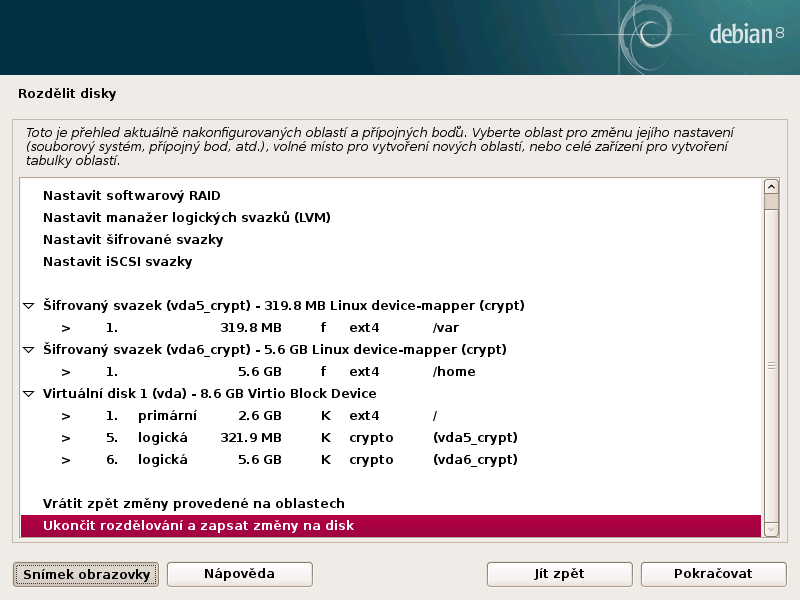
\includegraphics[width=.6\columnwidth]{pictures/debian1.png}
\end{figure}

\subsection{Ubuntu}

Ubuntu Linux vychází z~výše zmíněné distribuce Debian, instalátor však používá svůj vlastní. Je také jediným zástupcem linuxové distribuce, která využívá  schéma 
pro znázornění stavu rozděleného disku. Dříve využívané schéma programu GParted, které detailně rozebírám dále, bylo nahrazeno jednoduchou linkou v~horní oblasti okna instalátoru. Na této lince 
jsou barevně znázorněny diskové 
oddíly vytvořené uživatelem. Stejné barvy jsou poté použity u~každého ze záznamů v~seznamu oddílů, jak je možné vidět na obrázku č. 2. Tento jednoduchý diagram umožňuje rychlý odhad poměrů různých 
částí, které budou vytvořeny.

\begin{figure}[hb]
	\label{fig:ubuntu}
	\caption{Distribuce Ubuntu}
	\centering
	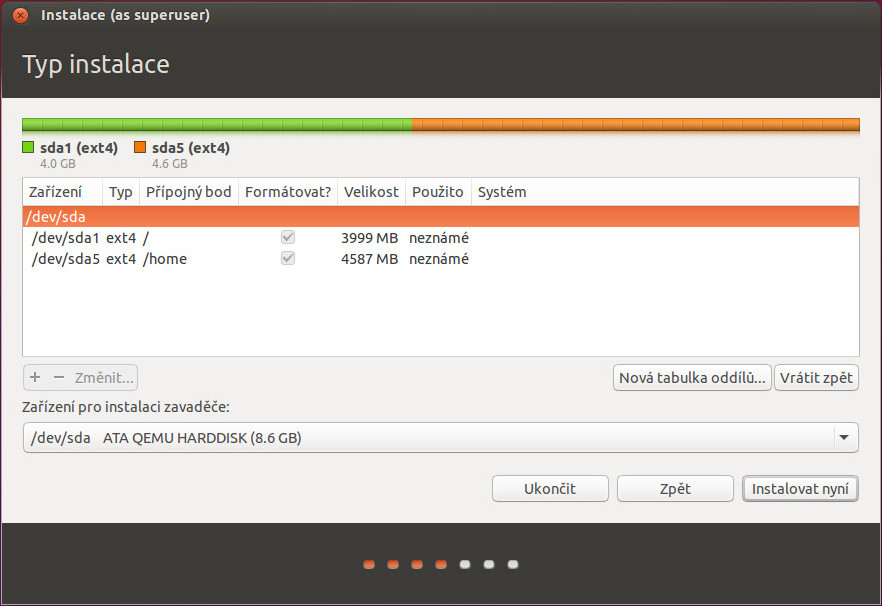
\includegraphics[width=.6\columnwidth]{pictures/ubuntu1.jpg}
\end{figure}

\subsection{CentOS}

Jako příklad systémů, které využívají instalátor Anaconda, jsem vybral systém CentOS. Tato zkratka znamená Community ENterprise Operating System. Na svých stránkách uvádějí \uv{The CentOS Linux
distribution is a~stable, predictable, manageable and reproducible platform derived from the sources of Red Hat Enterprise Linux (RHEL).}~\cite{CentOS}. Jedná se v~podstatě o~systém Red Hat Enterprise 
Linux, ovšem bez podpory a~oprav od společnosti Red Hat. V~současné době instalátor Anaconda používá také pouze textovou reprezentaci rozdělení disku. Rozdíl oproti ostatním distribucím tvoří 
seznam změn, který je zobrazen před finálním potvrzením a~započetím formátování. Na obrázku č. 3 můžeme vidět příklad tohoto seznamu. Situaci zpřehledňuje ale pouze pro malý počet změn, seznam s~mnoha 
záznamy o~změnách je nepřehledný. Zlepšením uživatelské přívětivosti při finální kontrole před instalací se zabývá tato práce.

\begin{figure}[h]
	\label{fig:centos2}
	\caption{Distribuce CentOS příklad souhrné tabulky}
	\centering
	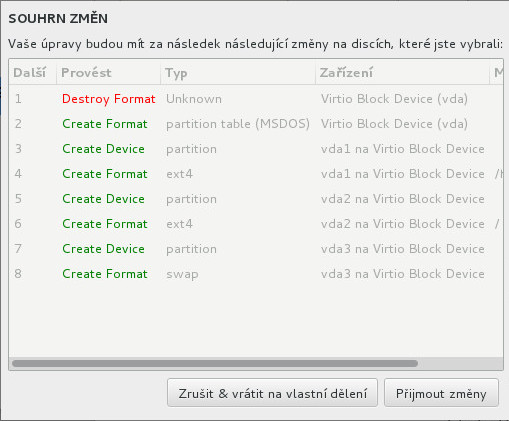
\includegraphics[width=.6\columnwidth]{pictures/centos3.jpg}
\end{figure}

\subsection{Windows 10}

Pro srovnání uvádím i~příklad nejrozšířenějšího systému, MS Windows. Vybral jsem v~současnosti nejnovější verzi, Windows 10. Překvapivě ani zde nejsou využity vizuální pomůcky.
Tvůrci instalátoru spoléhají na automatickou instalaci a~rozdělení disku s~tím, že pokročilou verzi s~manuálním nastavováním zvolí uživatel, který se zorientuje během instalace i~bez grafické nápovědy. 
Předchozí verze využívají stejný systém jako má distribuce Ubuntu, tj. obdélník znázorňující disk, v~němž jsou barevně vyznačeny diskové oddíly.

\begin{figure}[h!]
	\label{fig:win}
	\caption{Systém Windows}
	\centering
	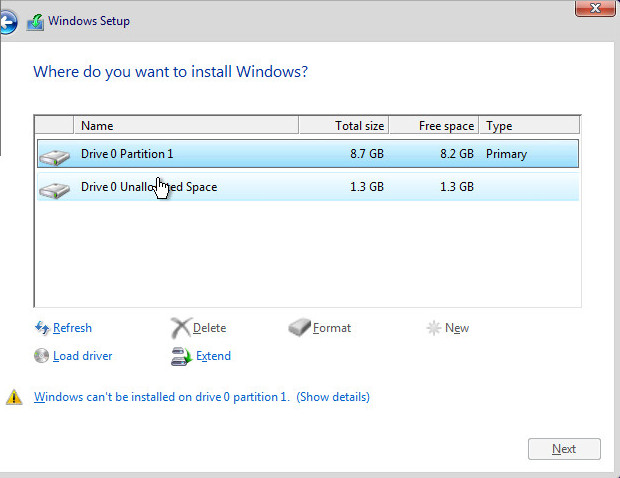
\includegraphics[width=.6\columnwidth]{pictures/win1.jpg}
\end{figure}

\section{Programy sloužící pro manipulaci s~disky}

\subsection{GParted}

Program GParted je zástupcem programů, které je možné spouštět i~mimo fázi instalace systému. Dříve byl součástí instálátoru systému Ubuntu, ale je možné jej spouštět i~samostatně, například 
 zvětšovat úložnou kapacitu virtuálních disků či disků, jejichž souborový systém umožňuje pozdější modifikaci. Opět je využito dříve zmíněné schéma obdélníku. Každý disk je reprezentovaný 
 obdélníkem a~další informace jsou zobrazovány barevnými rámci uvnitř těchto obdélníků. Narozdíl od ostatních zmíněných programů obsahuje GParted i~grafické aplikace pro manipulaci s~disky 
 a~tím dosahuje efektu WYSIWYG editoru (What You See Is What You Get, editor, který přímo ukazuje aktuální změny). Příkladem je aplikace pro zvětšení diskového oddílu, kterou vidíme na obrázku č.~5.

 \begin{figure}[h!]
	 \label{fig:gparted}
	 \caption{Ukázka widgetu pro program GParted~\cite{GParted}}
	 \centering
	 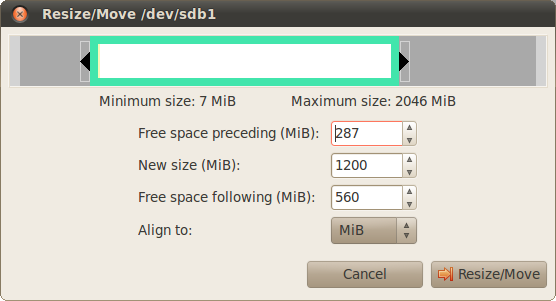
\includegraphics[width=.6\columnwidth]{pictures/gparted-5-big.png}\\
 \end{figure}

 \subsection{Blivet-gui}

 Druhým příkladem je program na manipulaci s~disky, využívá knihovnu nazvanou Blivet. Knihovna Blivet je dostupná ve všech systéch vycházejících ze systému RHEL. Autoři 
 se zprvu rozhodli použít známé schéma, avšak brzy narazili na problém s~větším počtem disků včetně virtuálních. Na obrázku č.~6 vidíme, že současné řešení je nedostatečné, jednotlivé úrovně barevných rámců 
 jsou znázorněny samostatnými uzly grafu s~hranami vyznačujícími vztahy mezi nimi. Mnoho těchto rámců uživatele spíše zmate a~použití grafu by situaci zpřehlednilo.

 \begin{figure}[h!]
	 \label{fig:blivet}
	 \caption{Ukázka programu blivet-gui~\cite{blivet-gui}}
	 \centering
	 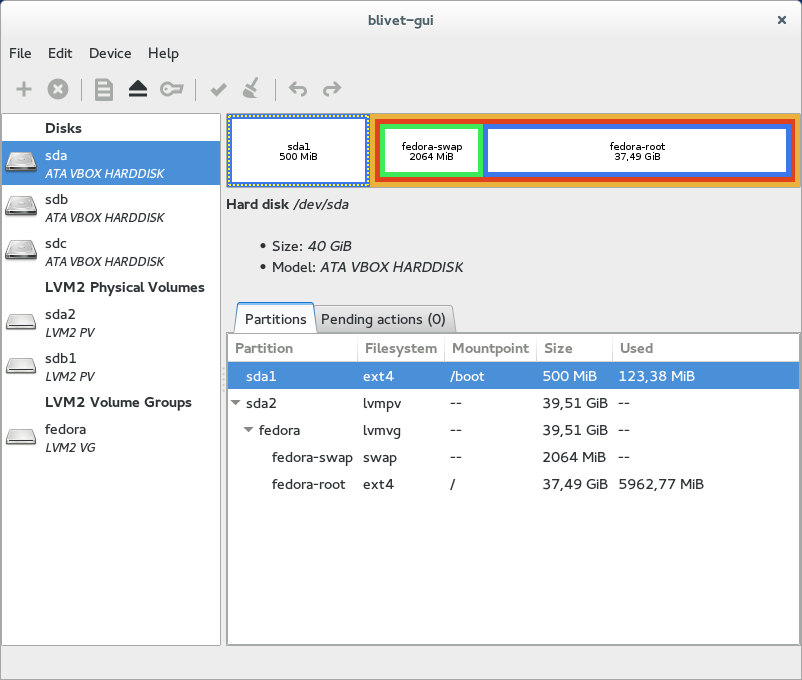
\includegraphics[width=.6\columnwidth]{pictures/blivet-gui-1.png}\\
 \end{figure}

\chapter{Použité knihovny}
\section{Knihovna Blivet}
	První a~nejdůležitější knihovou, která je v~mé práci využívána, je knihovna Blivet. Vznikla jako projekt
	ve firmě Red Hat, a~slouží k~rozšíření již zmiňovaného instalátoru Anaconda. Použití této knihovny je součástí zadání, a~proto nebudu diskutovat o jejích výhodách a~nevýhodách oproti ostatním knihovnám. 

	Mezi její funkce patří i~konfigurace různých datových úložišť, nemusí se jednat pouze o~pevné disky.
	Blivet ovládá i~mnohé další technologie, se kterými se lze v~dnešní době setkat. Příkladem jsou vícenásobná pole nezávislých disků (RAID), technologie logických svazků disku (LVM) či 
	ovládání zašifrovaných modulů pomocí technologie LUKS (Linux Unified Key System, systém pro správu klíčů v Linuxu). Všechny tři příklady rozebírám níže.

	Dále Blivet obsahuje nástroje pro práci se souborovými systémy diskových oddílů od starších, a~již dlouho používaných, jako jsou žurnálovací souborové systémy ext2 až ex4 či ReiserFS, po novější,
	jakým je Btrfs . Také se stará o~bootovací oddíly, čili master boot record (MBR) a~GUID partition table (GPT), tedy o~všechny součásti procesu přípravy 
	úložíšť v rámciinstalace
	nového systému na počítač.

\subsection{RAID}
	Vícenásobná pole nezávislých disků jsou velmi elegantní ochranou před selháním disků. Existůjí různé způsoby, jak pole realizovat, ale základní princip zůstává vždy stejný. 
	Několik disků, které vystupují jako jediný disk. Jedním z příkladů použití vícenásobného diskového pole může být disk s~kapacitou rovnou součtu disků, ze kterých je tvořen, anebo také
	kapacitou jednoho disku, přičemž data jsou zrcadlena na ostatní disky. Cílem tohoto nastavení je ochrana před selháním hardwaru a~ztrátou dat. 
	
	Blivet obsahuje nástroje pro práci se svobodným programem mdadm, která slouží k~nastavení softwarového pole MD RAID. Při využití hardwarových technologií, zvláště pak proprietárních,
	je možné k~tomuto RAIDu přistupovat jako k~obyčejnému disku, čehož i~nesvobodné RAIDy často využívají a~svých mnoho disků skrývají za jednotným rozhraním, které vystupuje jako jeden
	disk. 

	Program mdadm je softwarový RAID, a~proto má počítač celou dobu přehled nejen o~finálním disku, zabezpečeném proti selhání, ale i~o~všech dílčích discích, které ho tvoří. Výhodou
	softwarového RAIDu je
	možnost monitorování redundantních disků nástroji, které jsou součástí systému, bez nutnosti využívání aplikace třetích stran, u~kterých je hrozba nekompatibility, případně dalších 
	komplikací.
	Mezi nevýhody tohoto nastavení se řadí větší nepřehlednost při práci se všemi disky počítače, kdy změna jednoho disku vyvolá řetězovou reakci dalších změn. Právě proto je třeba data uceleně třídit
	a~pokud možno i~přehledně vizualizovat.

\subsection{LVM}
  LVM neboli Logical Volume Management je metoda, kterou je možné spravovat diskové oddíly. Poskytuje větší flexibilitu volného místa než klasické diskové oddíly a pracuje se třemi
	úrovněmi
	diskových zařízení. První úrovní jsou fyzické svazky neboli physical volumes (PV). Fyzický svazek je tvořen buď samotným diskem, včetně například disku RAID, nebo diskovým oddílem. 
	Fyzické
	svazky nenabízí o~mnoho více funkcionality než je označení a~příprava svazku pro další práci. Ta spočívá v~rozdělení fyzického svazku na fyzické extenty (physical extents, PE).

	Další úrovní jsou skupiny svazků (volume groups, VG), sdružující jeden nebo více fyzických svazků a logických svazků (LV). Skupiny svazků disponují úložným prostorem svých PV, 
	který rozdělují mezi LV. Výhodou existence VG je možnost libovolně přidávat svazky, a~to i~za plného chodu systému. Za chodu systému lze místo i~ubírat z VG, ale 
	pouze dosud neobsazenou část. 

	Třetí úrovní LVM jsou již zmíněné logické svazky, které jsou dostupné uživateli k~ukládání dat. Z~tohoto pohledu se chovají stejně jako obyčejné diskové oddíly. Jak již ale
	bylo zmíněno, výhodou oproti obyčejným diskovým oddílům je flexibilita dostupného místa. Na logických svazcích je možné vytvářet souborové systémy a~dále s~nimi pracovat.

	Kromě úprav velikosti oddílů za chodu je také možné přesouvat data v rámci VG. LVM také umí vytvářet snímky, tj. zachycovat stav dat v~čase. Využítí nachází tato 
	vlastnost
	při vytváření záloh a~jako záchytný bod, ke kterému je možné se vrátit. Nevýhodou LVM je skutečnost, že data na fyzických svazcích mohou být fragmentována, a~tak
	dochází ke snížení výkonu. Také je třeba mít na zřeteli fakt, že pokud zmenšujeme logický svazek, musí tuto funkci obsahovat i~souborový systém, který se na něm nachází.

\subsection{LUKS}
	Linux Unified Key Setup (unifikované nastavení klíčů na linuxu) zkráceně LUKS je specifikace šifrování disků původně vytvořená pro systém Linux. Existují i~implementace na jiné 
	systémy
	těmi se zde ale zabývat nebudu. LUKS vznikl, aby usnadnil proces nastavování šifrovaných dat, slovy autora : \uv{It has initially been developed to remedy the unpleasantness a~user 
	experienced that arise from deriving the encryption setup from changing user space, and forgotten command line arguments. The result of this changes are an unaccessible encryption
	storage.}\cite{on-disk-format} V~současné době se LUKS používá společně s~technologií dm-crypt, která slouží jako prostředek k~šifrování.

	Při využití LUKS v~Blivetu lze šifrovat disky, diskové oddíly, logické svazky i~fyzické svazky. Celé nastavení LVM může být šifrováno jedním klíčem, v součastnosti se takto 
	standardně šifruje LVM ve Fedora Linuxu, pokud uživatel nastaví automatické rozdělení disku s~šifrováním. Nemusí se jednat jen o~pevné disky, ale také o~odstranitelná média jako
	SD karty nebo USB paměti. Šifrovat lze též odkládací prostor paměti (swap).

\subsection{Formáty souborového systému}
  Jak již bylo zmíněno, Blivet umí pracovat i~se souborovými systémy. Struktura je následující. Výchozí seznam zařízení reprezentující jednotlivé disky, jejich oddíly a~případně
	speciální technologie jako RAID, LVM či šifrování LUKS. Každé zařízení má ale možnost mít i~formát, čímž se myslí formát souborového systému. Podporována je většina známých 
	souborových
	systémů, které jsou používány dlouhou dobu. Patří mezi ně souborový systém ext, ReiserFS, XFS. Taktéž existuje podpora pro Btrfs (B-tree FS), experimentální souborový systém 
	vlastněný společností Oracle. Přestože zatím u~Btrfs neexistuje stabilní verze, je mezi distribucemi podporován, neboť nabízí řešení některých problémů současných souborových systémů.

\section{Graphviz}
	Graphviz je program, který slouží k~vizualizaci dat formou grafů, orientovaných či neorientovaných. Pomocí Graphvizu je možné generovat grafy sloužící ke znázornění počítačové sítě nebo
	vztahů mezi určitými objekty. Nelze vytvářet grafy průběhů funkcí či grafy znázorňující vztahy mezi číselnými hodnotami. Jinými slovy Graphviz generuje grafy, jaké známe z~teorie grafů,
	ale není schopen generovat grafy známé například z~ekonomie.

	Program je z~velké části napsán v~jazyce C, ale ve existují obalovací knihovny (wrapper libraries) pro mnoho výšších programovacích jazyků. Vyššímy 
	programovacímy jazyky myslím jazyky, které jsou pokládány za méně náročné na obstarávání systémových věcí programátorem. Typickým příkladem výššího 
	programovacího jazyka je jazyk Java. Dalšímy příklady je Python a PHP. Často jsou tyto jazyky označovány jako skriptovací. 
	Z~těchto knihoven se budeme soustředit hlavně na
	knihovnu pro Python 3 která je používána v~mé práci. Pokud bychom Graphviz spouštěli jako program a~pracovali s~ním přímo například z~příkazové řádky, využívali bychom jeho vlastní jazyk
	na definici grafů nazvaný DOT. Tento jazyk je definovaný následovně:

	\uv{The following is an abstract grammar defining the DOT language. Terminals are shown in bold font and nonterminals in italics. Literal characters are given in single quotes. Parentheses
	( and ) indicate grouping when needed. Square brackets [ and ] enclose optional items. Vertical bars | separate alternatives.
	\begin{quotation}
	graph			:		[ \textbf{strict} ] (\textbf{graph} | \textbf{digraph}) [ ID ] \textbf{\'\\{\'} stmt\_list \textbf{\'\\}\'}
	stmt\_list :		[ stmt [ \textbf{';'} ] stmt\_list ]
	stmt			:		node\_stmt
	|							edge\_stmt
	|							attr\_stmt
	|							ID '=' ID
	|							subgraph
	attr\_stmt	:	(\textbf{graph} | \textbf{node} | \textbf{edge}) attr\_list
	attr\_list	:	'[' [ a\_list ] ']' [ attr\_list ]
	a\_list  	:	ID '=' ID [ (';' | ',') ] [ a\_list ]
	edge\_stmt	:	(node\_id | subgraph) edgeRHS [ attr\_list ]
	edgeRHS		:	edgeop (node\_id | subgraph) [ edgeRHS ]
	node\_stmt	:	node\_id [ attr\_list ]
	node\_id		:	ID [ port ]
	port			:	':' ID [ ':' compass\_pt ]
	|						':' compass\_pt
	subgraph	:	[ \textbf{subgraph} [ ID ] ] \textbf{'\\{'} stmt\_list \textbf{'\\}'}
		compass\_pt:	(\\textbf{n}| \\textbf{ne} | \\textbf{e} | \\textbf{se} | \\textbf{s} | \\textbf{sw} | \\textbf{w}  | \\textbf{nw} | \\textbf{c} | \\textbf{\_})}
	\end{quotation}

	Vidíme, že hlavnímy elementy při vytváření grafu jsou graf (graph), uzel (node) a~hrana (edge). Základní grafy lze tvořit jen pomocí těchto tří klíčových slov.

\subsection{Graf}
	Klíčové slovo graph uvádí jakýkoliv graf, který bude vytvořen, včetně prvního kořenového grafu. Každý zápis v~jazyce DOT musí začínat slovem graph nebo digraph. Výjimku tvoří užití slova
	strict, které se uvádí na začátku zápisu a které zamezuje vzniku vícenásobných hran, tedy mezi každým počátečním a koncovým uzlem bude jen jedna hrana. 

	Graph označuje graf neorientovaný, ve kterém jsou hrany bez šipek na koncích. Slovo digraph je zkrácené spojení directed graph (orientovaný
	graf) a~vyjadřuje graf orientovaný, ve kterém jsou na koncích hran šipky. Při vizualizaci rozdělení diskového prostoru jsem se rozhodl použít právě orientované grafy neboť, považuji za 
	důležité poskytnout uživateli co nejvíce vodítek ke znázornění vztahu rodič - potomek a~orientované hrany jsou ideální pro tento účel. 

	Speciálním případem grafu je podgraf (subgraph). Grafy mohou být vkládány do sebe a s~pomocí podgrafů lze snížit velikost zdrojového kódu v~jazyce DOT. Příkladem budiž situace, kdy zápisem
	hrany vedoucí od uzlu k~podgrafu ( A~-- \{B C\}) vytvoříme stejný efekt jako při zápisu každé jednotlivé dvojice mezi uzlem A~a~uzly B a~C (A~-- B, A~-- C). Dále je možné podgrafy využít
	pro specifikaci odlišných atributů uzlů či hran. V~podgrafu lze jednoduše nastavit jiné atributy než ve zbytku grafu.

	Poslední situací pro využití podgrafu je situace kdy chceme uzly shlukovat. V~tomto případě je nutné přidat k~názvu podgrafu klíčové slovo cluster a~určité grafovací algoritmy tyto uzly 
	uspořádají k~sobě do skupiny.

\subsection{Uzly}
	Uzly jsou základem každého grafu. V~graphvizu jsou definovány svým jménem. Základní graf s~jedním uzlem definujeme v~jazyce DOT jednoduše, a~to : graf \{A\}. Tento zápis vytvoří
	graf s~jedním uzlem uprostřed. Ve středu grafu bude napsán název uzlu, v~našem případě \uv{A}. Uzly mají mnoho různých atributů od svého jména po url odkazy a~atributy HTML formátování. 
	Nejdůležitějšími jsou ty které jsou definovány v~základním nastavení. Jsou to tvar uzlu (shape), barva výplně (fillcolor) a~jméno (name) nebo štítek (label). 
	
	Standardně je tvar nastaven na elipsu a~barva
	na bílou. Jméno se bere podle identifikátoru při vytváření uzlu, nálepka je rozšířením jména. Pokud je definována, nálepka nahrazuje jméno a~její obsah je vepsán dovnitř uzlu. Od jména se liší 
	tím, že její obsah lze libovolně upravovat, avšak lze do ní ukládat pouze text, jakékoliv speciální formátování nebude zohledněno. Pro vkládání obrázků slouží atribut image a~pro vkládání
	odkazů atribut url.

	Právě třemi základními atributy jsem se rozhodl rozlišovat jednotlivé typy zařízení, se kterými pracuje Blivet. S~pomocí tvaru uzlu odlišuji technologie zařízení. Čím je technologie
	abstraktnější, tím zaoblenější tvar má. Pevné disky a~jejich oddíly jsou znázorněny čtverci, LVM čtverci se zaoblenými rohy a~disky připojené přes síť či šifrování jsou znázorněny elipsou.
	Pro toto dělení jsem se rozhodl, abych zachoval konzistenci celého grafu a~pomohl uživateli rozlišit rozdíly jen pomocí krátkého shlédnutí tvaru.

	Druhým odlišovacím prvkem je barva, a to jak její odstín, tak sytost. Některé odstíny jsou rezervovány pro odlišení akcí, které budou provedeny při konfiguraci. Zelenou barvou jsou vyznačeny
	nově se objevivší prvky, červenou zaniknuvší prvky a~oranžovou prvky, u~kterých došlo ke změnám. Sytost barvy společně s~tvarem jasně definují použitou technologii. Barva pomáhá tam, kde
	samotný tvar nestačí. Čili pokud používá stejný tvar jak šifrování tak disk připojený přes internet, dojde k~jejich jednoznačnému odlišení použitím sytější a~méně syté barvy.

\subsection{Hrany}
	Hrany nejsou tak komplikovanými elementy jako uzly. Jejich základní atributy jsou počáteční a~koncový uzel. U~neorientovaného grafu se nerozlišuje, který uzel je počáteční. Hrany 
	nepoužívají tolik atributů jako uzly, avšak například nálepku stále mít mohou. Vzhledem k~jejich tvaru je u~nich zbytečný atribut výplňové barvy (fillcolor) a~používá se jen barva 
	\uv{pera}.
	Jak již bylo zmíněno, v~mé praci jsou všechny grafy orientované, a~tak záleží na pořadí v~jakém jsou uzly předány funkci, která tvoří hrany. Nicméně směr je vždy od rodiče k~potomkovi
	a~nikdy naopak.
	
\subsection{Rozložení}
	Graphviz nabízí různé možnosti rozložení grafu. Základních je pět, dot, neato, fdp, twopi, circo. Ke každému rozložení přikládám obrázek a~rozebírám jej 
	podrobněji. U~každého příkladu je použit stejný vstupní zápis, ale výsledky se velmi liší. Vstupní data vypadají takto:
	\begin{quotation}
	graph\{
		A~-- B
		B -- C
		C -- D
		D -- A
		D -- E
		D -- F
		G -- B
		G -- E
	\}
	\end{quotation}

	Prvním rozložením je rozložení dot. Oficiální dokumentace k~němu říká:
	\uv{dot - 'hierarchical' or layered drawings of directed graphs. This is the default tool to use if edges have directionality.}\cite{graphviz_layout} 
	Rozhraní dot přehledně udržuje hierarchii mezi rodiči a~potomky. Skládá
	své uzly do stromu, a~proto by mohl být kandidátem na použití v~mé práci. Lidé jsou zvyklí vnímat data ohledně úložného prostoru ve formě stromů. Tím pádem jde o~intiutivnější
	reprezentaci.

\begin{figure}
	\centering
	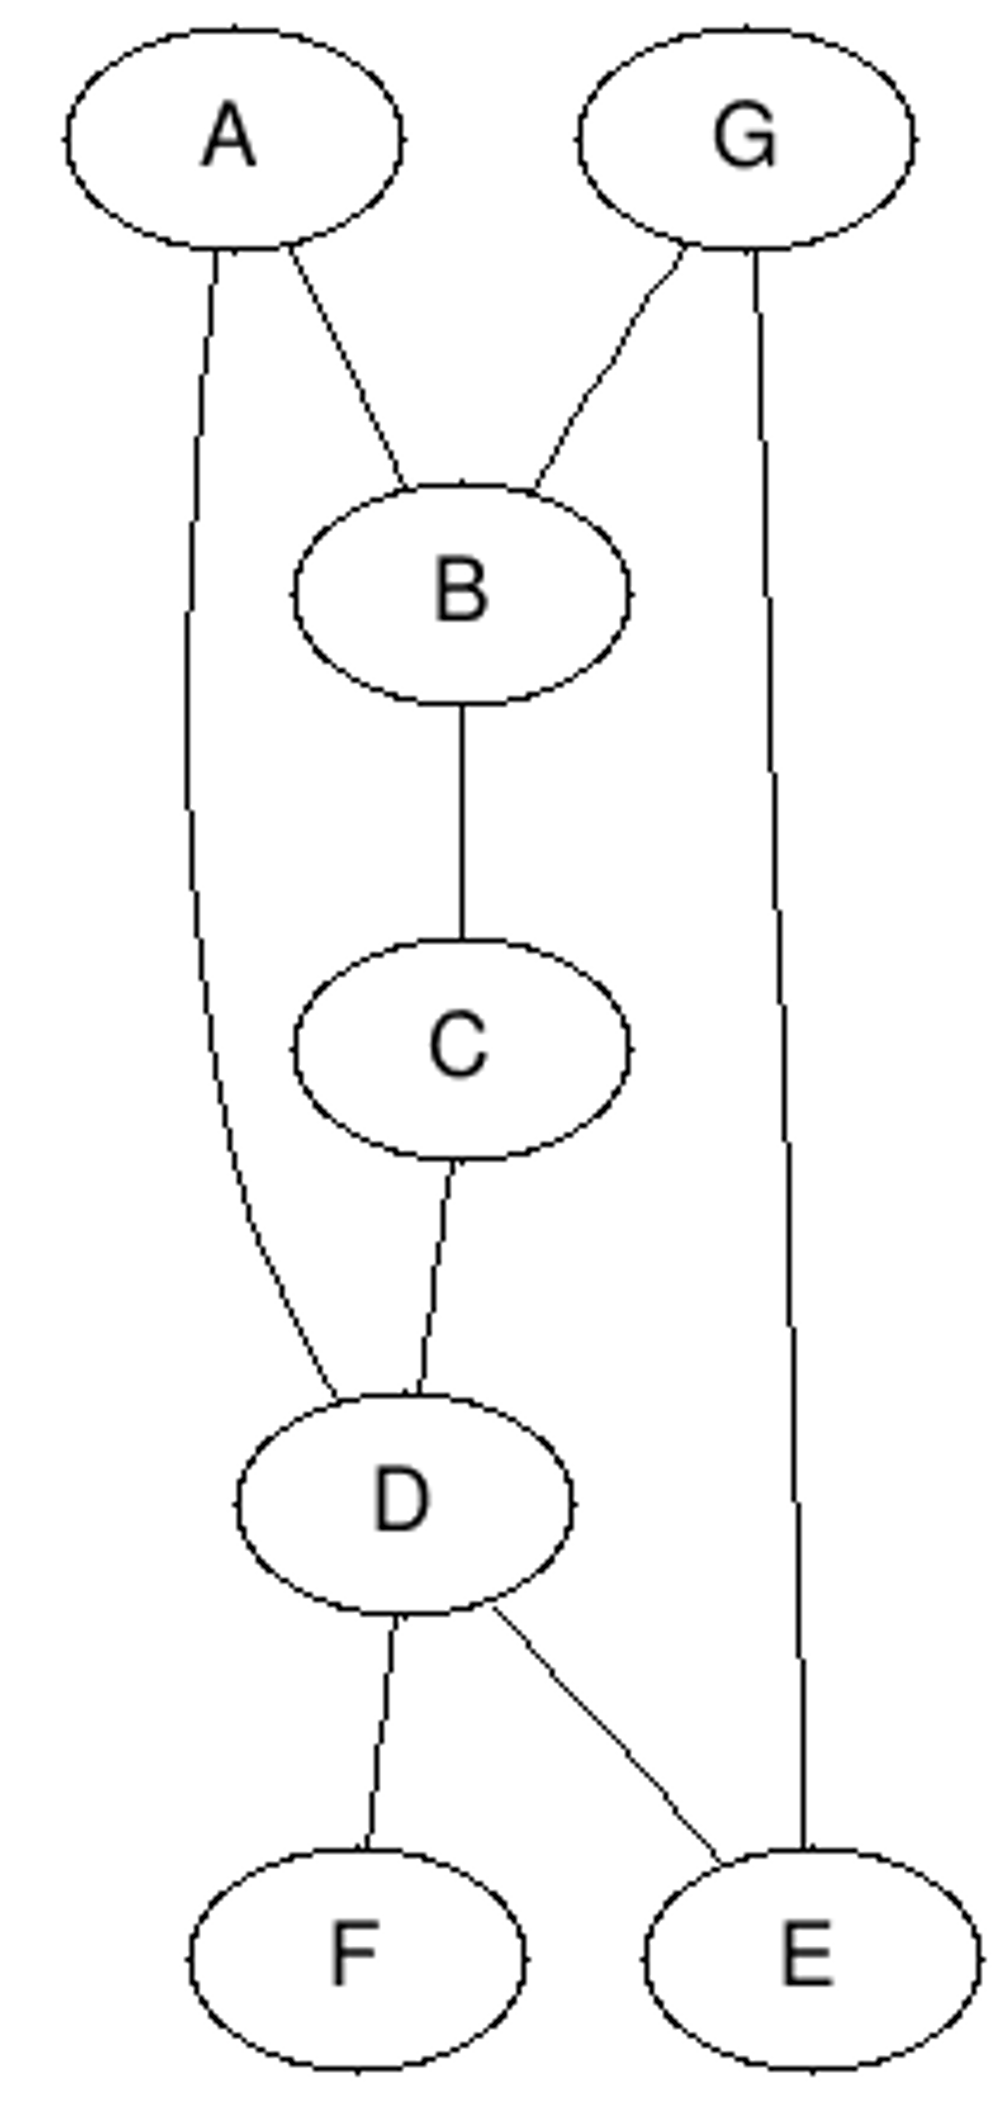
\includegraphics[width=0.6\textwidth]{pictures/dot_example.png} 
\end{figure}
	%TODO vysvětli globální energetickou funkci v grafech.
	Druhé rozložení, \uv{neato - 'spring model' layouts.  This is the default tool to use if the graph is not too large (about 100 nodes) and you don't know anything else about it. Neato attempts to
	minimize a~global energy function, which is equivalent to statistical multi-dimensional scaling.}\cite{graphviz_layout}
	Jinými slovy algoritmus neato se snaží vytvořit celý graf co nejmenší bez ohledu na ostatní faktory. Grafy nejsou hierarchické ani 
	strukturované. Cílem je co nejmenší zabraná plocha a~zároveň nepřekrývání hran a~uzlů. Kvůli chaotičnosti a~nestrukturalizovanosti se nejedná o~grafový algoritmus který bych mohl
	použít. Ostatně neato je přizpůsobeno na neorinetované grafy.
\begin{figure}
	\centering
	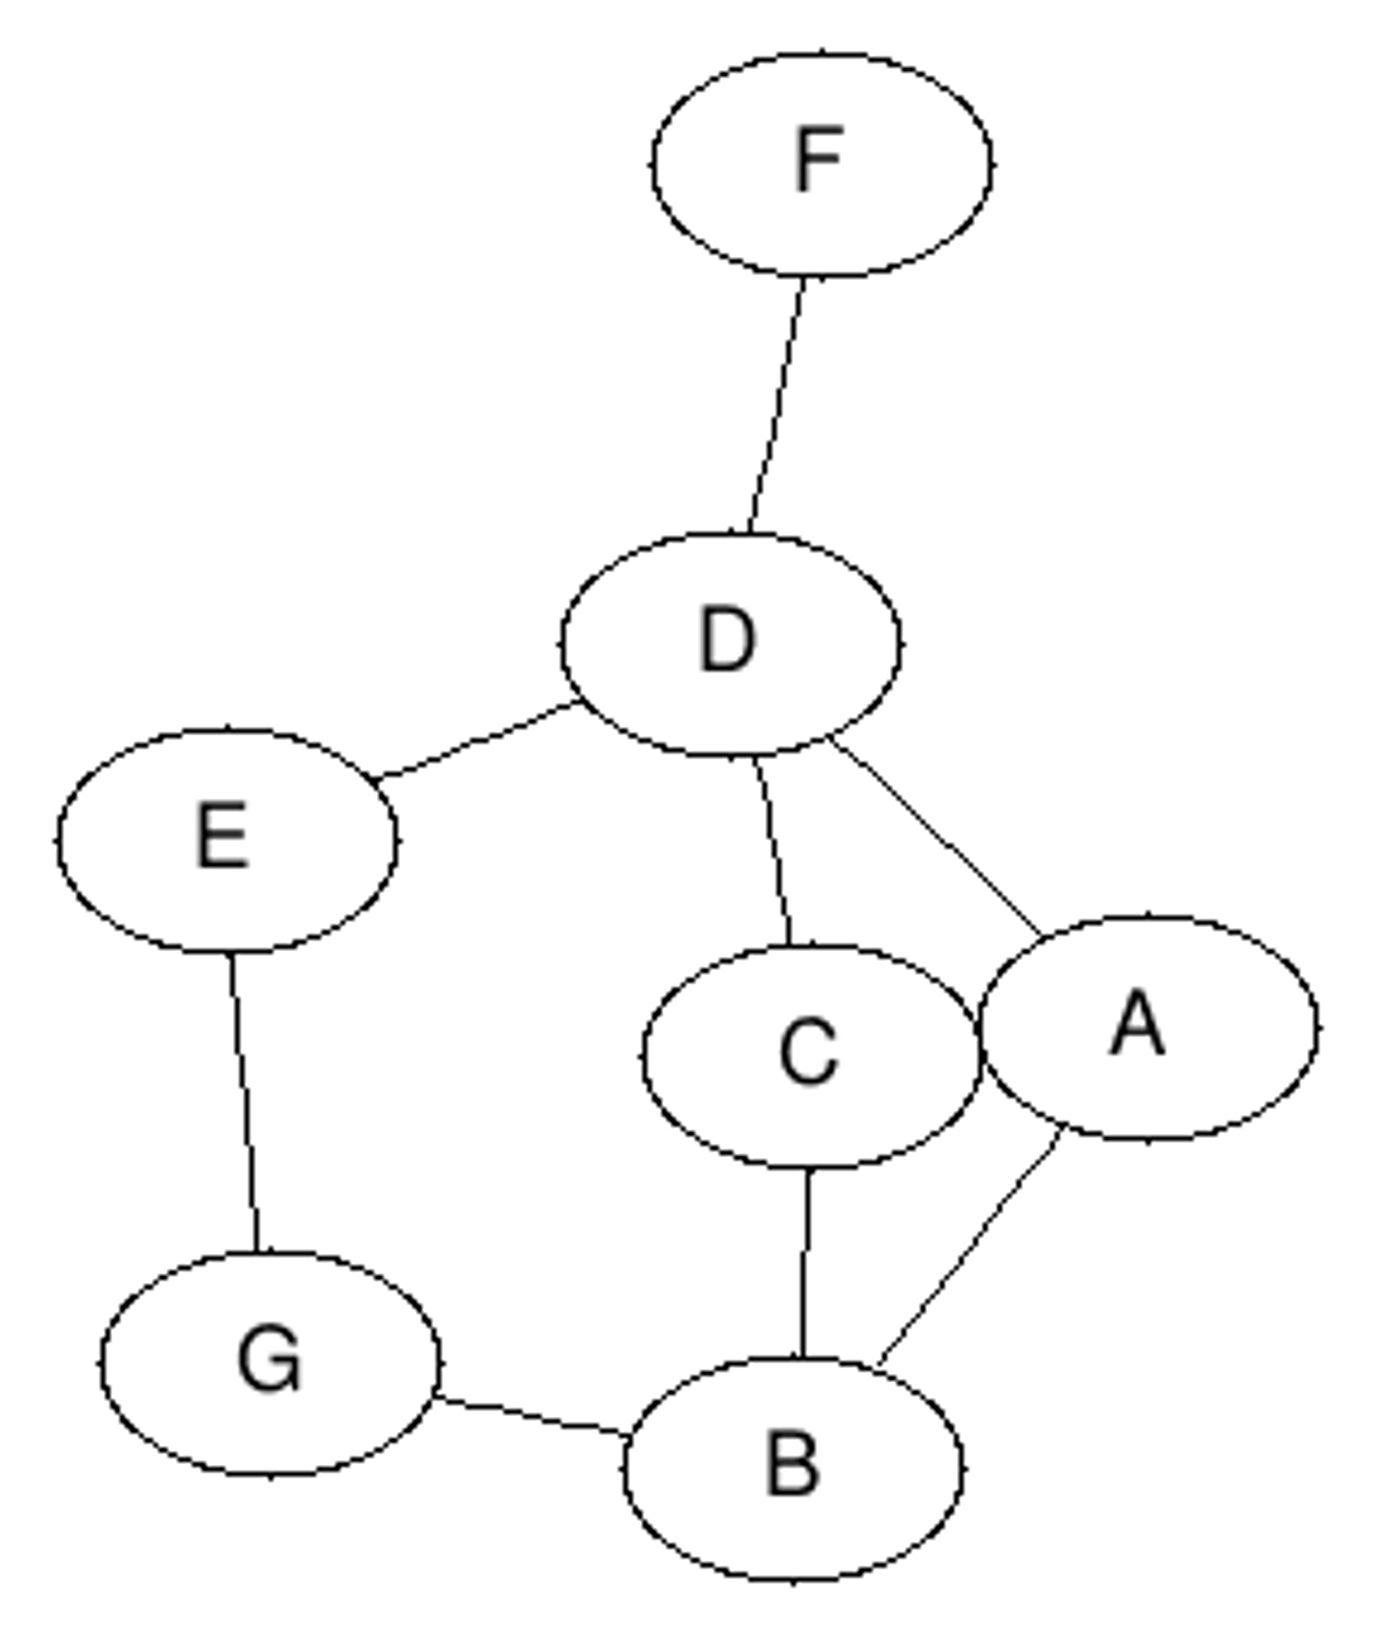
\includegraphics[width=0.6\textwidth]{pictures/neato_example.png} 
\end{figure}

	Třetí rozložení, \uv{fdp - 'spring model' layouts similar to those of neato, but does this by reducing forces rather than working with energy.}\cite{graphviz_layout} 
	Fdp je další z~rozložení pro neorientované grafy, ještě více zmenšuje plochu grafu, tentokrát i~s~ústupkem ohledně překrývání
	uzlů hranami. Pro grafy, které potřebuji vytvořit, se jedná o~ten nejhorší algoritmus z~pěti zde zmíněných. V~uzlech jsou zapsána data o~zařízeních a~hrany překrývající tyto uzly
	působí rušivě. Zároveň není třeba šetřit místem, neboť ve výsledné aplikaci je možné přibližovat a~posouvat graf dle libosti uživatele. Fpd tedy není algoritmem vhodným pro tuto
	situaci.
\begin{figure}
	\centering
	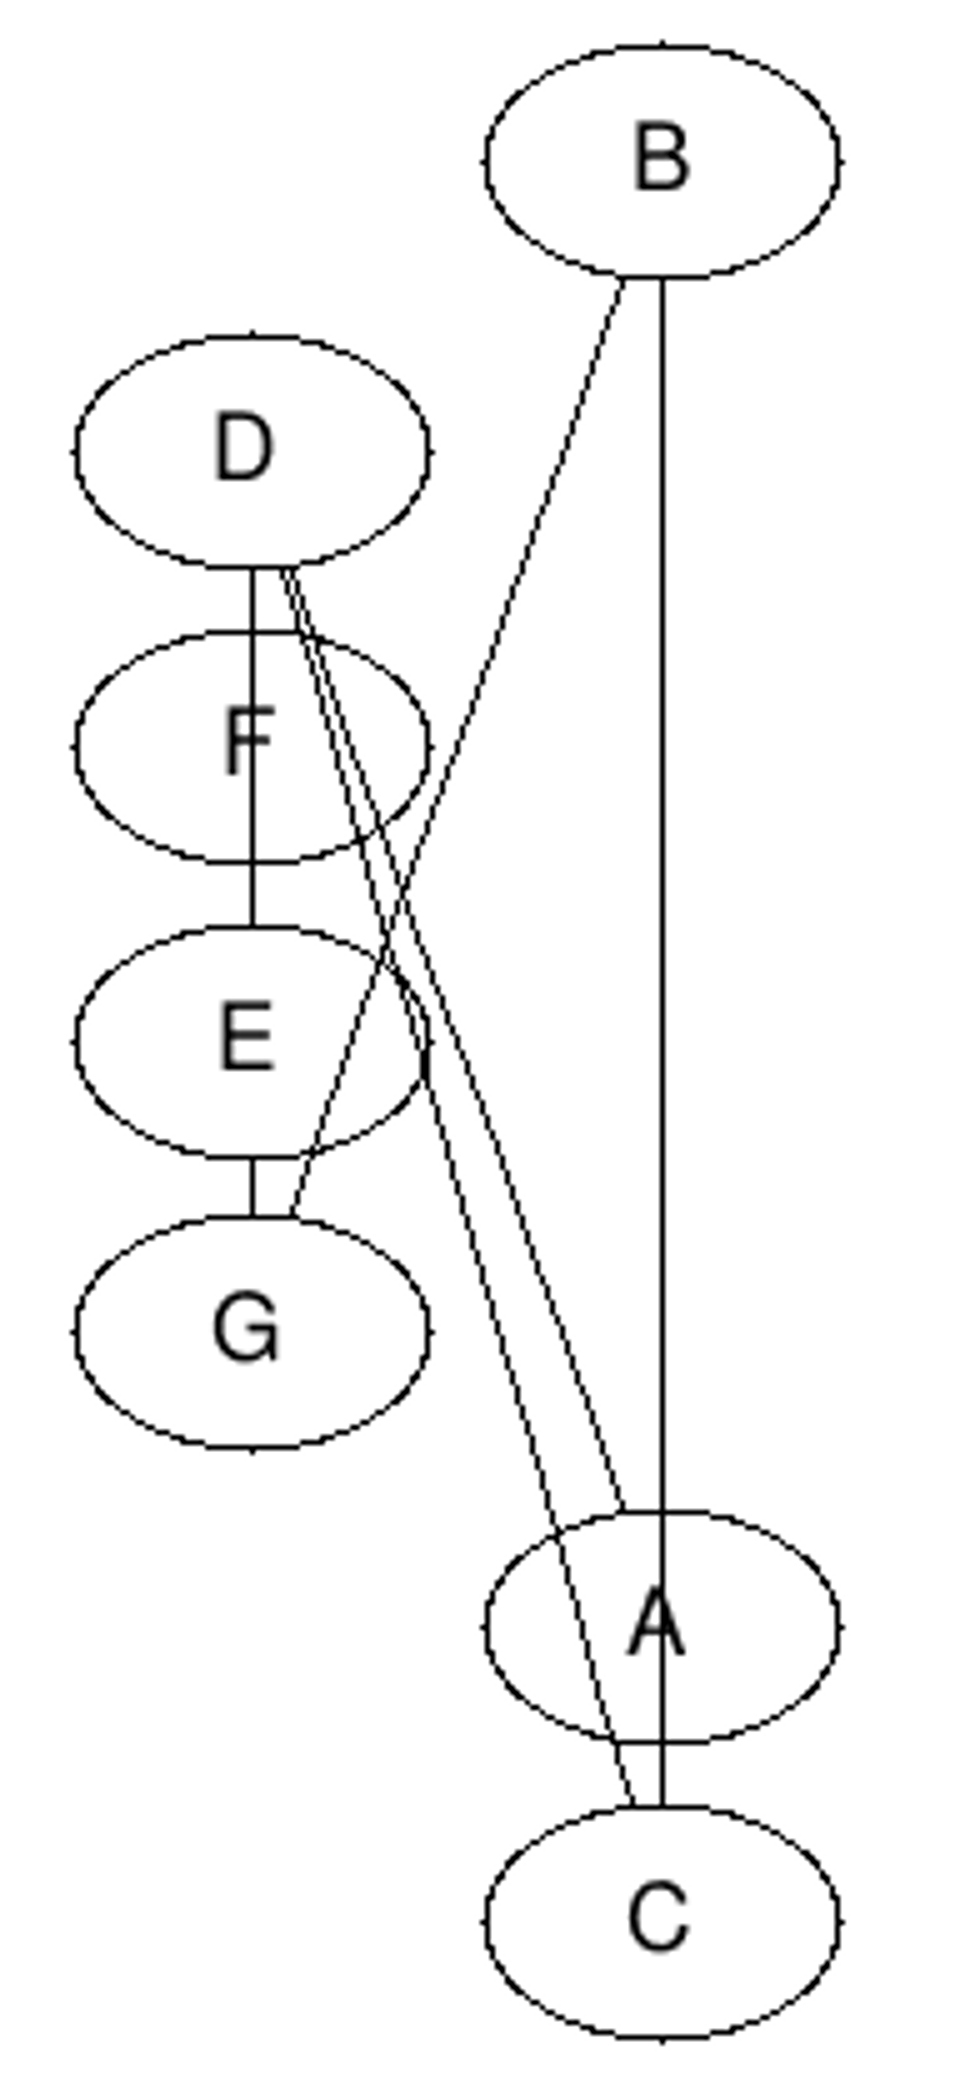
\includegraphics[width=0.6\textwidth]{pictures/fdp_example.png} 
\end{figure}

	Čtvrté rozložení, \uv{twopi - radial layouts.  Nodes are placed on concentric circles depending their distance from a~given root node.}\cite{graphviz_layout}
	Použitím paprskového rozložení dochází k~strukturalizaci grafu, tím pádem by se algoritmus twopi mohl zdát 
	dobrou volbou pro uskutečnění cíle, který jsem si vytyčil. Ovšem přidáním dalších dvou uzlů, které způsobí rozvětvení grafu, se strukturalizace začne vyvíjet neakceptovatelným směrem.
	Oba případy jsou vidět na obrázku. Strukturovanost do kruhů by, dle mého názoru, uživatele zbytečně mátla. Je důležité mít kořenový uzel, ovšem jeho umístění doprostřed je špatnou
	volbou.
\begin{figure}
	\centering
	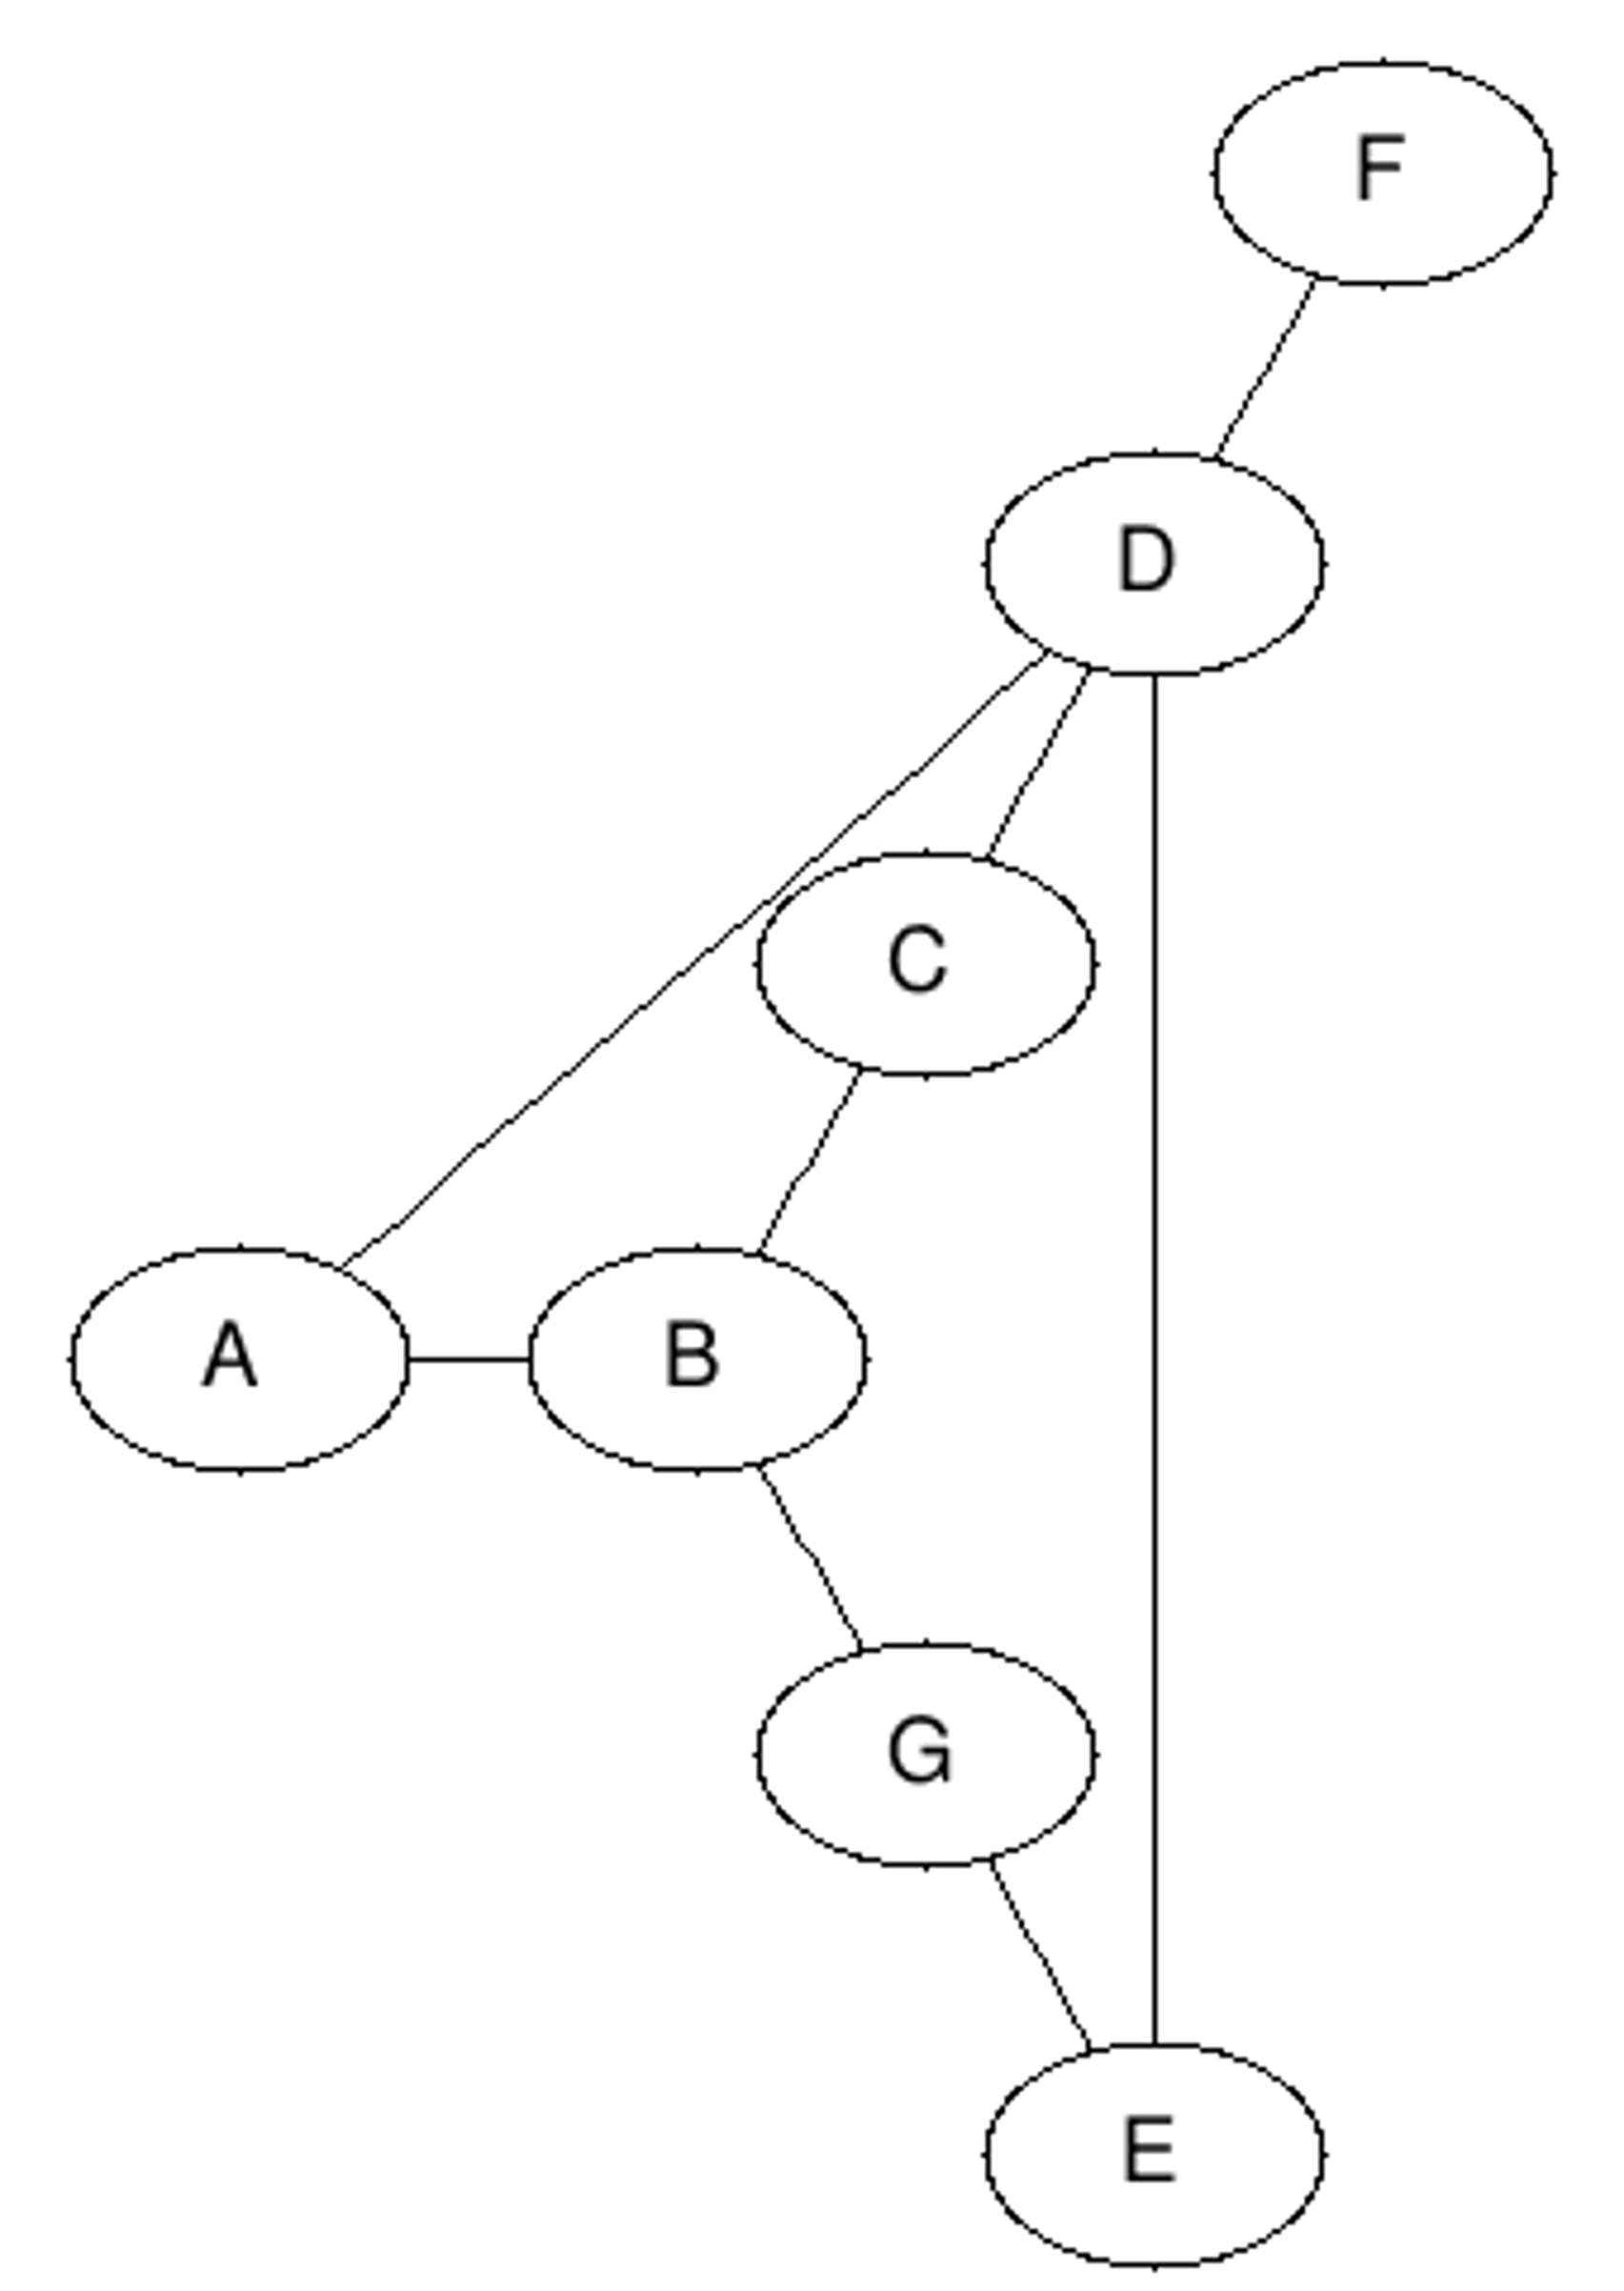
\includegraphics[width=0.6\textwidth]{pictures/twopi_example.png} 
\end{figure}
\begin{figure}
	\centering
	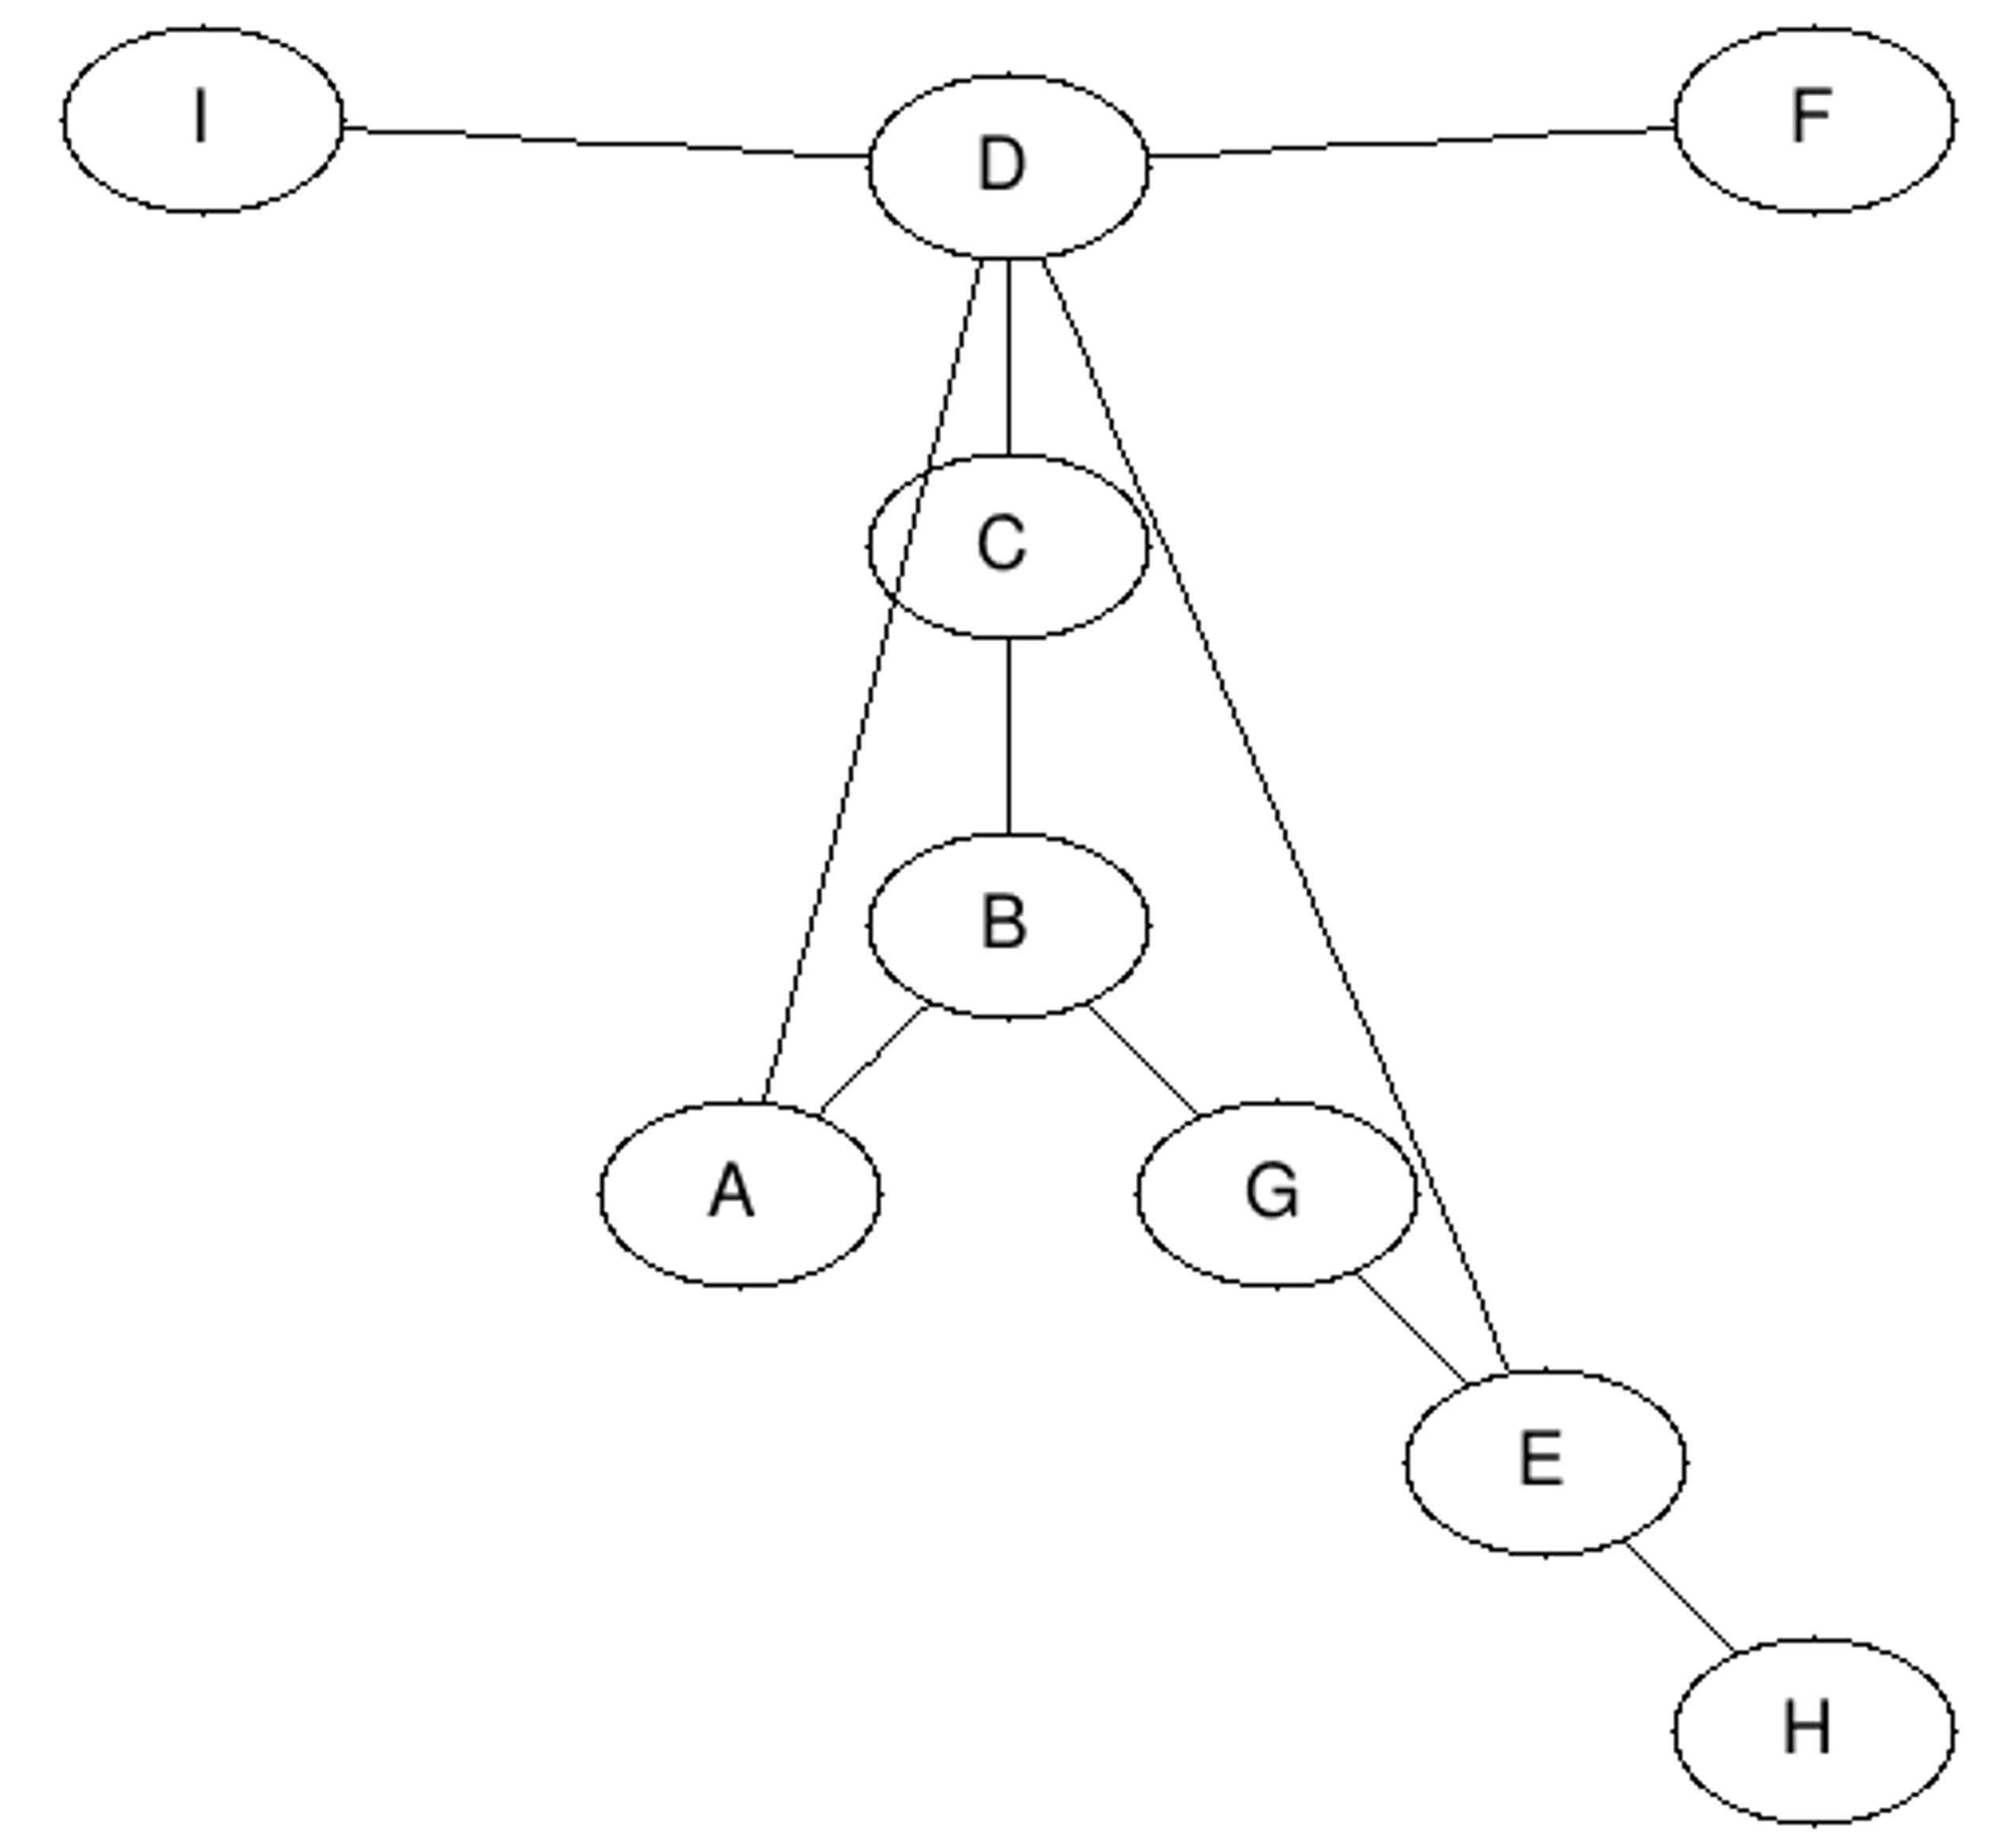
\includegraphics[width=0.6\textwidth]{pictures/twopi_example_2.png} 
\end{figure}

	Poslední rozložení, \uv{circo - circular layout. This is suitable for certain diagrams of multiple cyclic structures, such as certain telecommunications networks.}\cite{graphviz_layout} 
	Jak už je zmíněno v~dokumentaci, grafy používající rozložení 
	circo se hodí jen k~nemnoho specifickým účelům. Jak vidíme na obrázku, opět se setkáváme s~nehierarchickým grafem. Algoritmus circo rozhodně má své využití, ale ne v našem případě. V
	situaci, kdy připojujeme úložná zařízení v~systému Linux, se jen obtížně dostaneme do cyklických odkazů. Samotná podstata připojování úložných jednotek by měla zabraňovat těmto
	situacím. Pokud bychom už takovou situaci vytvořili, jedná se zcela určitě o~chybu buď používaných nástrojů, nebo chybu uživatelské konfigurace. 
\begin{figure}
	\centering
	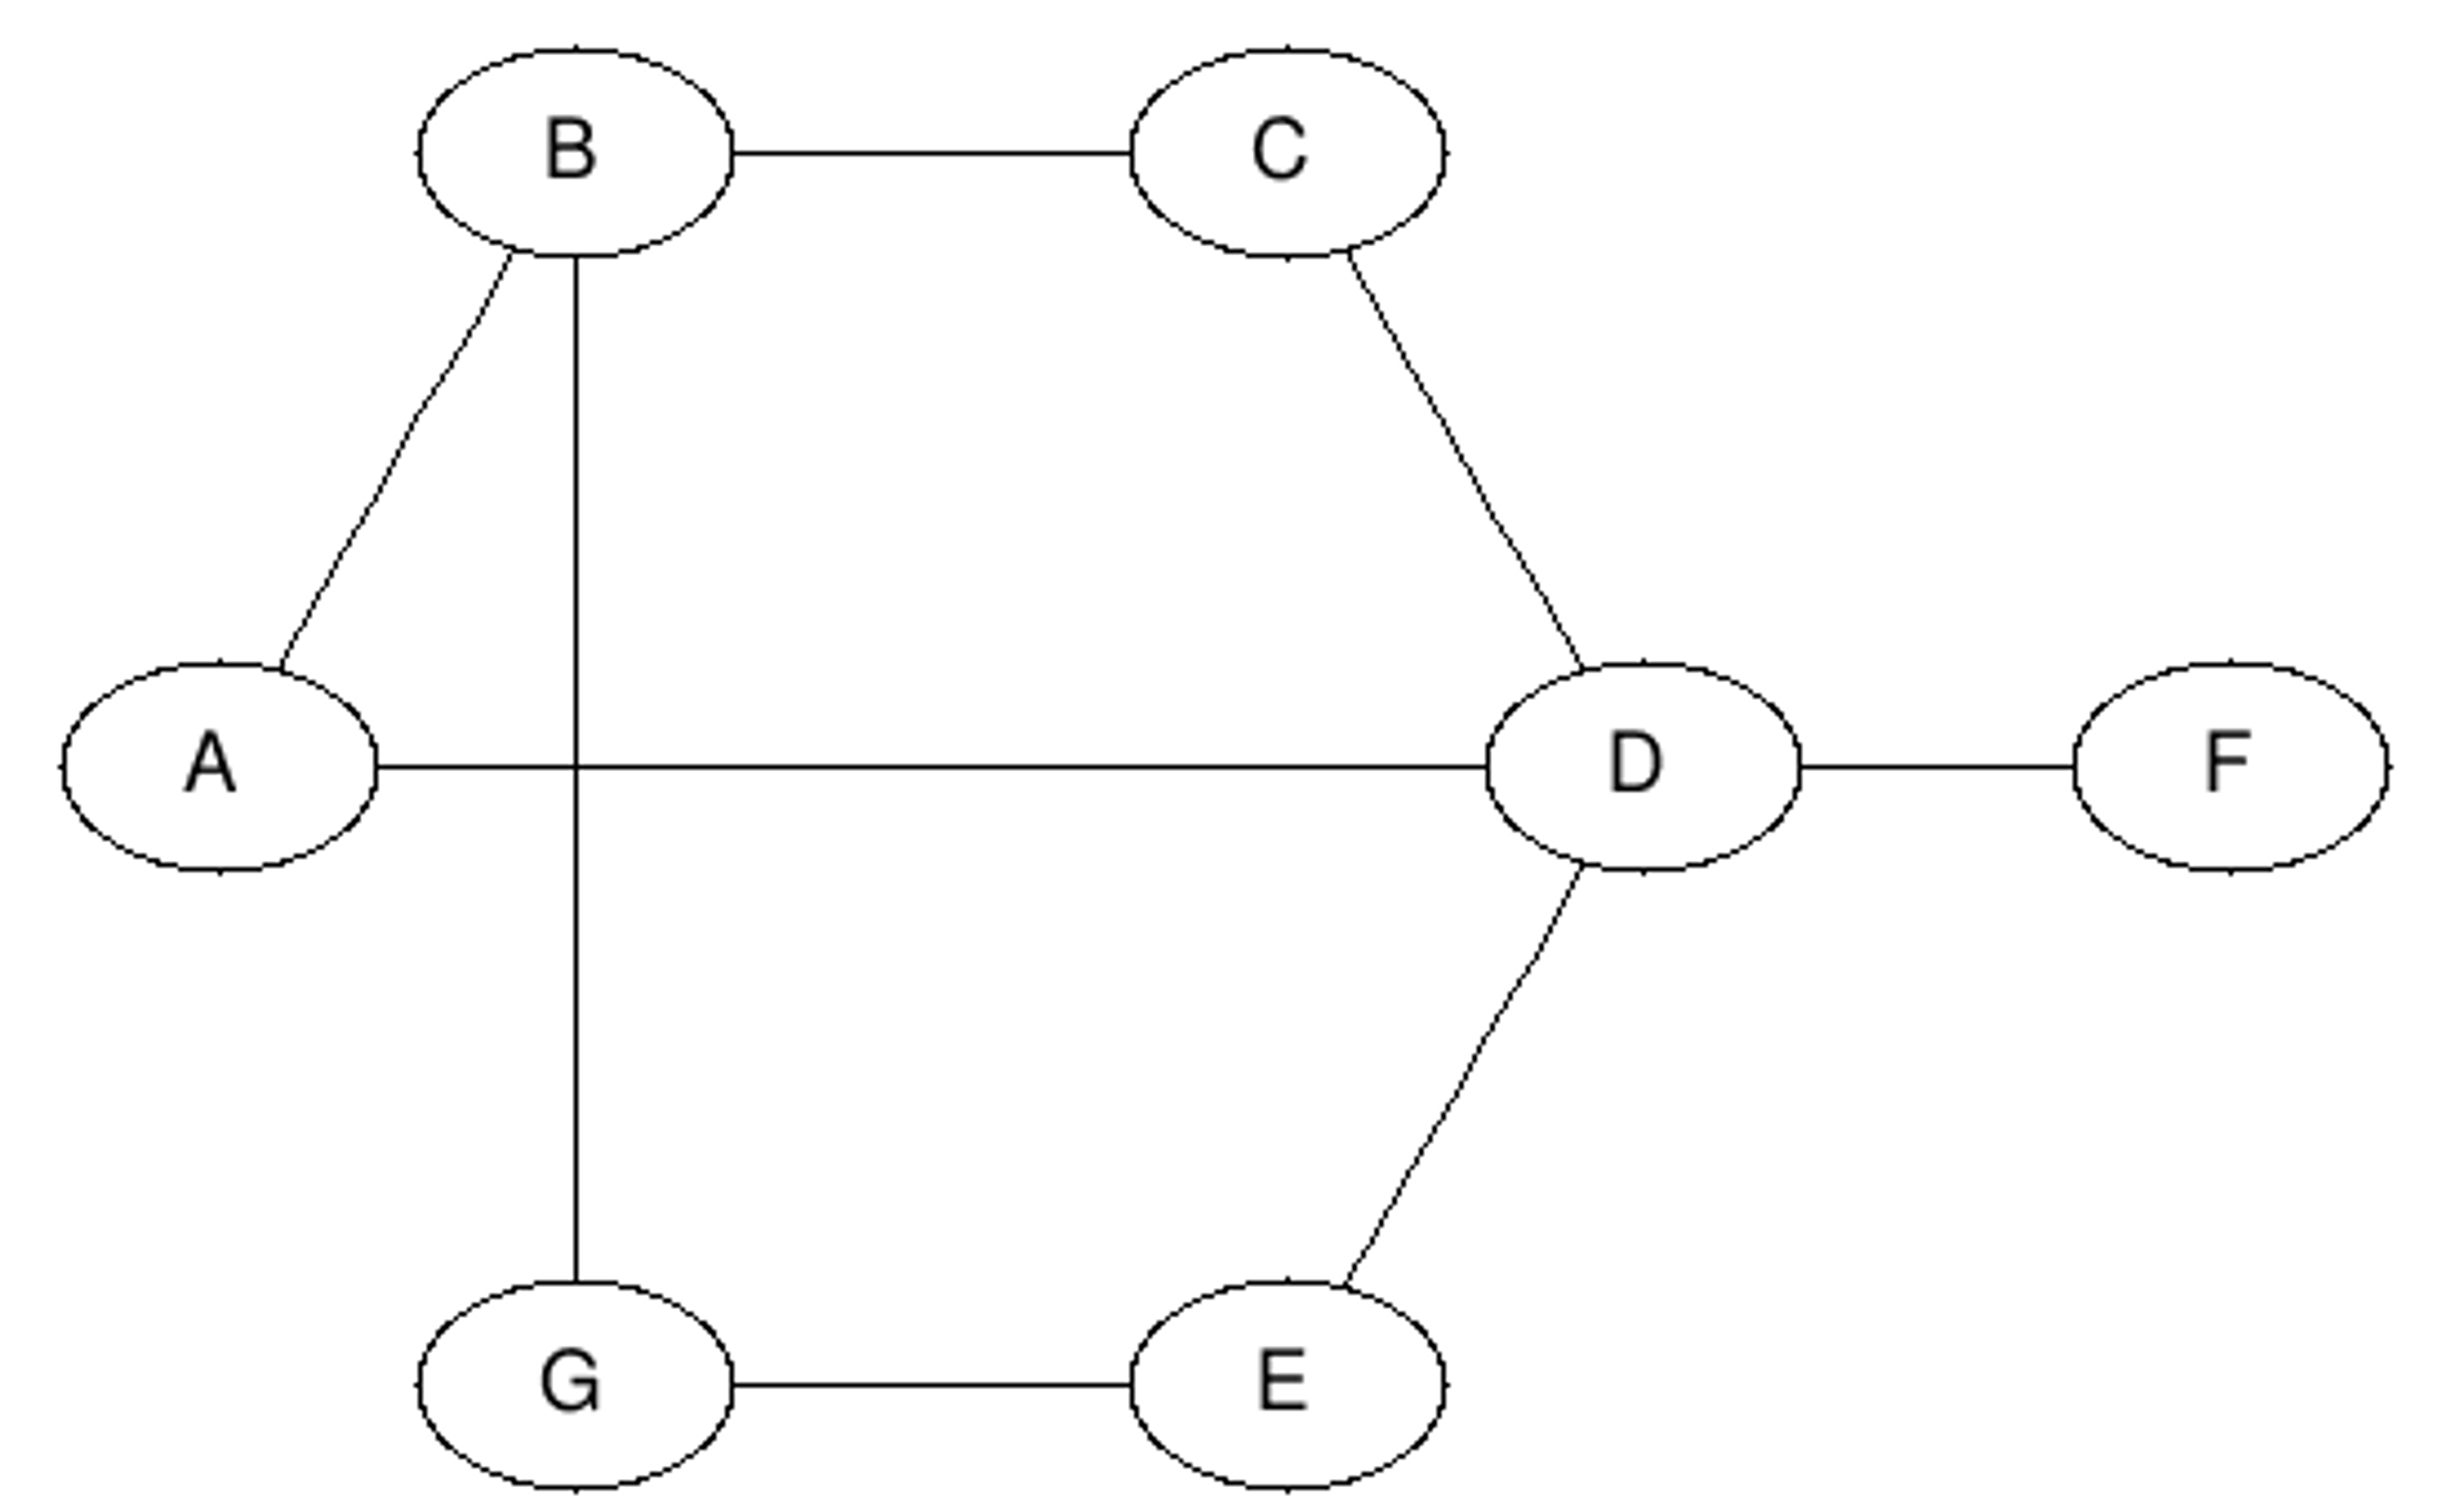
\includegraphics[width=0.6\textwidth]{pictures/circo_example.png} 
\end{figure}

	Algoritmem, který nakonec zbývá po aplikování vyřazovací metody, je algoritmus dot. 
	Základem pro mé rozhodnutí je stromová struktura. Ostatní typy rozložení nesplňují tuto podmínku, snad až na rozložení twopi. Twopi ale nelze použít kvůli větvení,
	ke kterému bude docházet velmi často. Navíc má problémy s~dměma a~více kořenovými uzly, nezařazuje je k~sobě, pokud nejsou spojeny hranou. V~prostředí, kde je využívána technologie
	RAID, jde o~zcela nepřijatelnou vlastnost. Je potřebné, aby disky logicky náležící k~sobě tak také byly vizualizovány. Jen dot splňuje tuto podmínku. Není problém směrovat grafy 
	vytvářené rozložením dot shora dolů či zleva doprava, zmíněné chování lze nakonfigurovat. Tím odpadá poslední argument pro použití twopi, které na prvním příkladě graf situuje jako
	jdoucí zleva doprava.

\chapter{Aplikace}
	Aplikace je napsaná v~jazyce Python a částečně využívá objektové paradigma. Důvody, které mě vedly k~výběru programovacího jazyka, jsou zmíněny v~úvodu práce. Za prvé, objekty logicky
	dělí program do částí, ve kterých se snadno orientuje a~které spolu souvisí. Tak jsou rozděleny i~mé třídy. Třída pro načítání dat, pro tvorbu grafu, pro uzly, pro hrany atd.
	Za druhé, objektové programovaní je dnes de facto standartem a~velká část nově vznikajících programů používá jazyky, které podporují objektové programovaní. Za třetí,
	objektové programování usnadňuje spolupráci a~čtení kódu ostatními programátory. Jelikož rozšiřuji svobodný software, je pravděpodobné že na něm někdo bude v~budoucnu pracovat
	a~rozšiřovat jej. Díky použití objektů bude mít usnadněnou práci.
	
\section{Třída Visualization}
	Hlavní třída mého programu je nazvaná Visualization, obsahuje základní atributy a~metody potřebné pro chod aplikace. Můžeme si ji představit jako centrální řídící jednotku. Ostatní
	třídy na ni navazují, ať už přímo nebo nepřímo (přes jinou třídu). 

	Konstruktor třídy visualisation vytváří dva seznamy, seznam uzlů a~seznam hran. S~oběma seznamy pracují hlavně funkce v~jiných třídách. Nejdůležitější funkcí
	je funkce create\_graph, která se dá volat z~příkazové řádky i~z~grafického rozhraní. Její argumenty jsou jméno a~cesta ke grafu a~výsledkem je soubor SVG obsahující graf. 
	V~případě spouštění z~grafického rozhraní okamžitě dojde k~zobrazení grafu v~okně aplikace, v~případě spuštění z~příkazové řádky jen k~jeho uložení v~definovaném adresáři. 

	Třída obsahuje i~pomocnou funkci prepare\_nodes, která prochází jednotlivě uzly v~seznamu uzlů, a~na každém spouští funkci prepare. Detailně funkci prepare rozebírám u~popisu uzlu. Funkce prepare\_nodes
	přemění data z~Blivetu na data vhodná pro graphviz. Textová data jsou utříděna, takže se vypíší, když uživatel rozklikne uzel. Funkci jsem přidal do této třídy proto, že 
	seznam uzlů je její atribut. Strukturu tohoto procesu bych chtěl nadále zachovat i~po dalším rozšíření.  

\section{Třída pro načítání dat}
	Třída pro načítání dat, GvInput, slouží k~načítání dat z~Blivetu, naimportuje si Blivet jako modul a vytvoří si objekt obsahující veškeré informace
	o~blokových zařízeních. Verze knihovny Blivet 2.0.0 vyžaduje před 
	každým načítáním dat spustit funkci reset(). Tato funkce projde dostupné úložné kapacity a~vytvoří strom zařízení (device\_tree). Stejně tak naplní i~seznam těmi
	samými objekty. Můj program projde tímto seznamem (Blivet.devices) a~u~každého prvku nejdříve zkontroluje, zda se nenachází na černé listině. Na ní se nachází věci jako jsou 
	výměnná média, která jsou při instalaci zbytečná a~jen by na grafu překážela.

	Dalším krokem je vytvoření objektu reprezentujícho uzel grafu, jeho zpracování a~přidání do vlastního seznamu uzlů, který funguje jako převodník mezi Blivetem a~graphvizem. Při
	přidávání do seznamu se uzly zároveň třídí pomocí přepínače a~jsou jim nastavovány barvy a~tvary. Vše, co potřebujeme pro zobrazení uzlu, se ukládá ihned při průchodu seznamem. 
	Tím dosáhneme pouze jediného průchodu. Uzly si už pak informace zpracují samy. V~případě, že by uzel nebyl rozpoznán, nenastane situace, kdy by program 
	zhavaroval. Jednoduše 
	se při vytvoření použije přednastavená barva a~tvar (bílá, elipsa).

	Nastavování tvarů a~barev je řešeno obdobně jako užití příkazu switch v~jazyce C či podobných. Python tento výraz přímo neobsahuje, a~tak jsem byl nucen použít funkci obsahující 
	sérii if příkazů. Po vyhodnocení jedné z~větví na hodnotu pravda se spustí jiná funkce,která nastavuje vzhled uzlu. Konkrétní příklad, na seznamu je diskový oddíl. Není na blacklistu,
	proto postupuje dál. Konstruktoru třídy Node jsou předány informace z~Blivet.device. Poté je uzel předán funkci process\_node, která jej rozpozná jako oddíl, a~spustí funkci 
	nodeIsPartition. V~ní je výsledný uzel obarven světlou barvou a~je mu nastaven tvar box, neboli tvar s~ostrými rohy. Poté je uzel přidán do seznamu node\_list. Také je na
	standardní výstup vypsána hláška o~přidání nového členu seznamu. Uživatel tak má přehled, které uzly jsou přidány. Zařízení je identifikováno svým jménem a~typem.

	Po přidání uzlu se přidávají hrany. U~každého uzlu program projde seznam jeho rodičů a~vytvoří od nich hrany zpět k~právě vytvářenému uzlu. 
	Knihovna Blivet nemá jiné propojení mezi zařízeními než seznam rodičů. Stále ale stačí projít seznam zařízení jen jednou. Hrana se vytváří pomocí koncových uzlů, které má spojovat.
	Pokud jeden chybí, je vytvořen. Opět nedochází k~havárii programu. Pokud už uzel existuje je k~němu hrana připojena. Pokud uzel neexistuje je později, až přijde na řadu, obarven.

\section{Třída Node}
	Třída pro uzly je poměrně jednoduchá, obsahuje převážně metody pro nastavení vzhledu. Nejdůležitější informace se ukládají už v~konstruktoru, jako ochrana opět slouží nastavení
	prázdných řetězců tam, kde by vstupní informace chyběly. Kromě konstruktoru obsahuje třída Node také funkce change\_color a~change\_shape nastavující vzhled. K~funkci change shape 
	jsem vytvořil i~pomocnou funkci change\_style\_safely. Pomáhá vytvořit styl uzlu se zakulacenými rohy. Graphviz řeší tuto situaci přidáním klíčového slova rounded k~už 
	existujícímu stylu. Pokud je styl nastavený na obdélník s~ostrými rohy (box), je třeba přidat slovo rounded a~obě slova oddělit čárkou. Výsledek musí vypadat takto \uv{box, rounded},
	přičemž na pořadí slov nezáleží.

	Ukládání atributů a~gv\_atributů (atributů pro graphviz) je řešeno pomocí slovníků. Použití slovníků umožňuje libovolně přidávat a~ubírat počty atributů. 
	Atributy rozumíme informace o~nastavení úložných zařízení, které se později vypisují ke každému uzlu. Jedinou výjimku tvoří jméno a~typ zařízení, neboť jde
	o~identifikační atributy a~jejich neexistence by znemožnila fungování programu. Rozhodl jsem se oddělit atributy pro knihovnu graphviz do samostatného slovníku. Díky tomu je při
	vykreslování grafu možné jen projít záznamy a~vytvořit z~párů klíč, hodnota páry atribut ulzu hodnota v~grafu. 

	Poslední pomocnou funkcí nacházející se v~tříde Node je fukce prepare. Připravuje textová data pro prezentaci ve formě grafu. Projde všechny záznamy ve slovníku attributes a~spojí je do 
	jednoho řetězce obsahujícího znaky nového řádku. Před spojením je možné flexibilně měnit počet a~obsah textových informací. Poté co je spuštěna funkce prepare, je její výsledný řetězec
	uložen do atributu gv\_atribute label a~je připraven pro použití Graphvizem.

\section{Třída Edge}
	Třída pro hrany obsahuje konstruktor a~funkce pro získání počátečního a~koncového uzlu. Konstruktor bere za své argumenty právě tyto dvě 
	proměnné. Proměnnou node\_from, počáteční uzel a~proměnnou node\_to, koncový uzel. I~přesto, že neobsahuje moc funkcí, jsem se rozhodl vytvořit dedikovanou třídu pro hrany. 
	Takto je pro každý element v~grafu dedikovaná třída, se kterou lze pracovat.

\section{Třída pro vytváření grafů}
	Samotné vytváření grafu také není ničím zvlášť složitým, nicméně pro použití v~mé aplikaci je potřeba výsledný graf dále upravit. Rozeberme funkce ve ve třídě output chronologicky,
	tak, jak jsou použity. Tradičně konstruktor přebírá seznam uzlů a~hran. Volá funkci vytvářející graf se jménem createGvGraph a~předává jí své argumenty. 

	CreateGvGraph nejprve vytvoří orientovaný graf pomocí graphvizu. Poté projde seznam uzlů a~pomocí graphvizu vytvoří všechny uzly v~nově utvořeném orientovaném grafu. To samé udělá i
	s~hranami. Funkce pro vytváření uzlů graphviz.node bere jako první argument jméno uzlu. První argument je povinný, jméno uzlu. Povinný je argument jména
	i~při vytváření v~seznamu uzlů. Druhý argument ze tří je atribut label. Jde o~dlouhý řetězec rozdělený znaky dalších řádků, jak je vysvětleno výše v~částí věnující se třídě Node.
	Poslední argument je seznam zbylých atributů, které dokáže graphviz zobrazovat. Je předán jako celý seznam a~po jeho rozbalení se aplikují nastavení vzhledu uzlu. Na konci je celý
	graf vrácen návratovou hodnotou.

	Druhá funkce se nazývá createSvg. Jejím úkolem je přepsat graf do formátu SVG. Používá funkci pipe z knihovny Graphviz. Pipe dokáže vytvářet i~jiné formáty, ale ty nejsou v~tuto
	chvíli důležité. Formát svg byl vybrán proto, že v~něm lze použít JavaScript, a~tím dosáhnout interaktivity. Konkrétně se jedná o~možnost zvětšovat uzly, posouvat a~přibližovat graf.
	Popis funkcí následuje později, níže rozebírám postup implementace.

	Skript v JavaScriptu vkládá pomocná funkce insert\_JS\_to\_graph, přebírající jeden argument, a~to řetězec obsahující svg grafu, do kterého se má vložit zmíněný skript. Řetězec je výstupem funkce
	graphviz.graph.pipe s~argumentem format="svg". 

	Funkce insert\_JS\_to\_graph nejprve nastaví výchozí jmenný prostor (namespace; funkcionalita XML jazyků schopná rozlišovat různé elementy se stejným názvem) z~ns0 na prázdný 
	řetězec. Svg by bylo validní i~se jmenným prostorem ns0 nicméně standardně po vygenerování knihovnou graphviz tento jmenný prostor není přítomen a~považuji za lepší do svg 
	zasahovat co nejméně. 

	Dále se svg nahraje do objektu ElementTree (ET). ET je obsažen v~základní knihovně jazyka Python, je jednou ze tříd pro práci s~daty ve formátu XML. Vytváří v~paměti stromovou
	strukturu totožnou s tím, jak je reprezentována načteným XML souborem. Obsahuje funkce pro čtení rodičů i~potomků, funkce pro vytváření, přidávání a~mazání elementů a~vyhledávání pomocí 
	XPath. Element Tree lze nahrát ze souboru či z~řetězce. V aplikaci využívám funkci načítání z~řetězce. Poté vybírám kořenový element a~upravuji jeho atributy.

	Úpravou atributů se rozumí přidání odkazu na xmlns:xlink, kvůli možnosti odkazovat na soubory s~JavaScriptem. Také je třeba odstranit atribut viewBox, aby mohlo fungovat posouvání
	grafu. Zároveň je třeba připravit atribut viewport u~prvního potomka elementu svg. První potomek je kořenový uzel zobrazovaného grafu, vždy nese id graph0. Pomocí XPath výrazu je
	nalezen a~je mu  přiřazen zmíněný atribut.

	Poté už stačí jen vytvořit nový element s~cestou k~JavaScriptovému souboru a~tento element přidat jako prvního potomka kořenového elementu svg. Funkce insert\_JS\_to\_graph vrací celý
	Element Tree.

	Po návratu z~funkce insert\_JS\_to\_graph použijeme metodu write k~zapsání svg do souboru, kde je svg připraveno k~zobrazení.

\section{Třida Gui}
	Můj program lze používat jak dávkově z~příkazové řádky, tak interaktivně s~pomocí grafického uživatelského prostředí. Dávkový režim nabízí pouze možnost vygenerovat graf v~určitém 
	umístění. Interaktivní režim nabízí možnost graf ihned prohlížet. Variací na interaktivní režim je také okno s~grafem, které se zobrazuje při instalaci, jako vizualizace změn prováděných
	instalátorem. 

	Třída gui obsahuje vše potřebné pro obsluhu uživatelského rozhraní. Je naprogramována s~pomocí nejrozšířenější linuxové knihovny pro uživatelská rozhraní Gnome toolkit (GTK). Jde o~
	obyčejné okno s~několika tlačítky. Jsou v~ní obsaženy ovládací prvky potřebné pro nastavení umístění grafu, tlačítko pro vyvolání kontextové
	nápovědy a~plocha zobrazující samotný graf. Pro zobrazení grafu je použita technologie WebKit. Okno WebKitu je možné vložit do GTK aplikace a~tím dosáhnout stejné základní funkcionality,
	jakou mají dnešní moderní webové prohlížeče. V~mém případě jde o~schopnost zobrazit svg a~schopnost spouštět JavaScript.

	Rizikem, které je nutné přijmout, je možná známá zranitelnost prohlížečů a~nutnost ukládat soubor svg na disku. WebKit totiž zobrazuje svg s~pomocí protokolu file://. Počítač se
	tak ptá sám sebe na existenci souboru v~určité cestě definované uživatelem, a~pokud jej najde, zobrazí jej uživateli. Pokud by se k~systému dostal útočník, mohl by soubor upravit a~
	zanechat v~něm škodlivý kód. Nicméně bezpečnost systému není věcí této práce a~vychází se z~předpokladu, že systém, na kterém je vizualizace spouštěna, je buď ve fázi instalace, nebo
	je již zabezpečen. WebKit je de facto prohlížeč, který je možné vložit do GTK aplikace.

\chapter{Návrh vzhledu}
TBD

\chapter{Závěr}
TBD
\section{Další možnosti rozšiřování}
	Zadání mé práce je schváleno jako dostatečné pro bakalářskou práci. Přesto jsem během vypracování diskutoval o další možné nadstavby a~pokračování v~práci.

	První rozšíření by byla možnost vytvářet XML soubory obsahující informace z~grafů. Již existuje aplikace schopná vytvářet XML soubory z~Blivetu a~zase je zpět nahrávat. Jeho zamýšlené
	použití je vytváření záchytných bodů, ke kterým je možné se vrátit v~případě havárie instalátoru, přerušení dodávky elektrického proudu či jiné fatální chyby systému. Ideou pro export
	XML z~grafu je možnost na systém přenést tu konfiguraci, která je prezentována.

	Druhým a~ambicióznějším rozšířením je schopnost grafu fungovat jako samostatný konfigurační nástroj. Graf by nejenom zobrazoval data, která mu byla poskytnuta, ale také by je byl
	schopen upravovat a~předávat nová data zpět aplikaci Blivet, popřípadě instalátoru. Například by bylo možné přesouvat logické oddíly LVM mezi PV jednoduchým 
	přetažením myší stejně, jako dnes kopírujeme soubory přetažením jejich ikony. Nové oddíly by byly vytvářeny také přetažením z~nějaké nabídky předpřipravených uzlů. Konkrétní velikosti
	a~jména zařízení by se editovaly s~pomocí textových polí v~každém uzlu.
	
	Největším problémem, který by bylo třeba vyřešit, je načítání svg a~informací z~něj zpět zároveň s~ukládáním informací z~prohlížeče. 
	Jedním z~možných postupů by byla úprava XML načítače tak, aby fungoval i~pro svg graf zobrazovaný uživateli. Uživatel by přetvořil graf podle svých představ, poté spustil 
	konfiguraci, a~ta by přenesla stav do Blivetu a~provedla změny v~úložném prostoru systému. 

	\printbibliography

\end{document}
